%\documentclass[twoside]{article}
\documentclass{article}
% If your paper is accepted, change the options for the package
% aistats2019 as follows:
%
%\usepackage[accepted]{aistats2019}
\usepackage{amssymb}
\usepackage{algorithm}
\usepackage{caption}
\usepackage{amsmath}
\usepackage{amsthm}
\usepackage{graphicx}
\usepackage{subfigure}
\usepackage{tabularx}
\usepackage{pifont}
\usepackage[noend]{algpseudocode}
\usepackage{bm}
\usepackage{array}
\usepackage{balance}
\usepackage{amsthm}
\usepackage{amsmath}
\usepackage{amssymb}
\usepackage{multirow}
\usepackage{fullpage}
\usepackage{color}

\def\rc{\color{red}}
\def\bc{\color{blue}}

\usepackage[colorlinks,linkcolor=red,citecolor=blue]{hyperref}       % hyperlinks
\usepackage{natbib}
\allowdisplaybreaks
 
\DeclareMathOperator*{\Argmax}{Argmax}
\DeclareMathOperator*{\Argmin}{Argmin}

\newcommand{\var}{{\rm var}}
\newcommand{\Tr}{^{\rm T}}
\newcommand{\vtrans}[2]{{#1}^{(#2)}}
\newcommand{\kron}{\otimes}
\newcommand{\schur}[2]{({#1} | {#2})}
\newcommand{\schurdet}[2]{\left| ({#1} | {#2}) \right|}
\newcommand{\had}{\circ}
\newcommand{\diag}{{\rm diag}}
\newcommand{\invdiag}{\diag^{-1}}
\newcommand{\rank}{{\rm rank}}
\newcommand{\expt}[1]{\langle #1 \rangle}
% careful: ``null'' is already a latex command
\newcommand{\nullsp}{{\rm null}}
\newcommand{\tr}{{\rm tr}}
\renewcommand{\vec}{{\rm vec}}
\newcommand{\vech}{{\rm vech}}
\renewcommand{\det}[1]{\left| #1 \right|}
\newcommand{\pdet}[1]{\left| #1 \right|_{+}}
\newcommand{\pinv}[1]{#1^{+}}
\newcommand{\erf}{{\rm erf}}
\newcommand{\hypergeom}[2]{{}_{#1}F_{#2}}
\newcommand{\mcal}[1]{\mathcal{#1}}
\newcommand{\Rcal}{{\mathcal{R}}}
\newcommand{\Acal}{{\mathcal{A}}}
\newcommand{\Ccal}{{\mathcal{C}}}
\newcommand{\Fcal}{{\mathcal{F}}}
% boldface characters
\renewcommand{\a}{{\bf a}}
\renewcommand{\b}{{\bf b}}
\renewcommand{\c}{{\bf c}}
\renewcommand{\d}{{\rm d}}  % for derivatives
\newcommand{\e}{{\bf e}}
\newcommand{\f}{{\bf f}}
\newcommand{\g}{{\bf g}}
\newcommand{\h}{{\bf h}}
\newcommand{\bi}{{\bf i}}
\newcommand{\bj}{{\bf j}}
\newcommand{\bK}{{\bf K}}
\newcommand{\Kcal}{{\mathcal{K}}}
% in Latex2e this must be renewcommand
\renewcommand{\k}{{\bf k}}
\newcommand{\m}{{\bf m}}
\newcommand{\mhat}{{\overline{m}}}
\newcommand{\tm}{{\tilde{m}}}
\newcommand{\n}{{\bf n}}
\renewcommand{\o}{{\bf o}}
\newcommand{\p}{{\bf p}}
\newcommand{\q}{{\bf q}}
\renewcommand{\r}{{\bf r}}
\newcommand{\s}{{\bf s}}
\renewcommand{\t}{{\bf t}}
\renewcommand{\u}{{\bf u}}
\renewcommand{\v}{{\bf v}}
\newcommand{\w}{{\bf w}}
\newcommand{\x}{{\bf x}}
\newcommand{\y}{{\bf y}}
\newcommand{\z}{{\bf z}}
\newcommand{\bl}{{\bf l}}
\newcommand{\A}{{\bf A}}
\newcommand{\B}{{\bf B}}
\newcommand{\C}{{\bf C}}
\newcommand{\D}{{\bf D}}
\newcommand{\Dcal}{\mathcal{D}}
\newcommand{\E}{{\bf E}}
\newcommand{\F}{{\bf F}}
\newcommand{\G}{{\bf G}}
\newcommand{\Gcal}{{\mathcal{G}}}
\renewcommand{\H}{{\bf H}}
\newcommand{\I}{{\bf I}}
\newcommand{\J}{{\bf J}}
\newcommand{\K}{{\bf K}}
\renewcommand{\L}{{\bf L}}
%\newcommand{\Lcal}{{\mathcal{L}}}
\newcommand{\M}{{\bf M}}
\newcommand{\Mcal}{{\mathcal{M}}}
\newcommand{\N}{\mathcal{N}}  % for normal density
%\newcommand{\N}{{\bf N}}
\newcommand{\bupeta}{\boldsymbol{\upeta}}
\renewcommand{\O}{{\bf O}}
\renewcommand{\P}{{\bf P}}
\newcommand{\Q}{{\bf Q}}
\newcommand{\R}{{\bf R}}
\renewcommand{\S}{{\bf S}}
\newcommand{\Scal}{{\mathcal{S}}}
\newcommand{\T}{{\bf T}}
\newcommand{\Tcal}{{\mathcal{T}}}
\newcommand{\U}{{\bf U}}
\newcommand{\Ucal}{{\mathcal{U}}}
\newcommand{\tU}{{\tilde{\U}}}
\newcommand{\tUcal}{{\tilde{\Ucal}}}
\newcommand{\V}{{\bf V}}
\newcommand{\W}{{\bf W}}

\newcommand{\Ocal}[1]{{\mathcal{O}\left( #1  \right)}}
\newcommand{\Omegacal}[1]{{\Omega \left( #1 \right)}}
\newcommand{\Pcal}{{\mathcal{P}}}
\newcommand{\Hcal}{{\mathcal{H}}}
\newcommand{\Wcal}{{\mathcal{W}}}
\newcommand{\X}{{\bf X}}
\newcommand{\Xcal}{{\mathcal{X}}}
\newcommand{\Y}{{\bf Y}}
\newcommand{\Ycal}{{\mathcal{Y}}}
\newcommand{\Z}{{\bf Z}}
\newcommand{\Zcal}{{\mathcal{Z}}}

% this is for latex 2.09
% unfortunately, the result is slanted - use Latex2e instead
%\newcommand{\bfLambda}{\mbox{\boldmath$\Lambda$}}
% this is for Latex2e
\newcommand{\bfLambda}{\boldsymbol{\Lambda}}

% Yuan Qi's boldsymbol
\newcommand{\bsigma}{\boldsymbol{\sigma}}
\newcommand{\balpha}{\boldsymbol{\alpha}}
\newcommand{\bpsi}{\boldsymbol{\psi}}
\newcommand{\bphi}{\boldsymbol{\phi}}
\newcommand{\bbeta}{\boldsymbol{\beta}}
\newcommand{\bepsi}{\boldsymbol{\epsilon}}
\newcommand{\Beta}{\boldsymbol{\eta}}
\newcommand{\btau}{\boldsymbol{\tau}}
\newcommand{\bvarphi}{\boldsymbol{\varphi}}
\newcommand{\bzeta}{\boldsymbol{\zeta}}

\newcommand{\blambda}{\boldsymbol{\lambda}}
\newcommand{\bLambda}{\mathbf{\Lambda}}

\newcommand{\btheta}{\boldsymbol{\theta}}
\newcommand{\bTheta}{\boldsymbol{\Theta}}
\newcommand{\bpi}{\boldsymbol{\pi}}
\newcommand{\bxi}{\boldsymbol{\xi}}
\newcommand{\bSigma}{\boldsymbol{\Sigma}}
\newcommand{\bPi}{\boldsymbol{\Pi}}
\newcommand{\bOmega}{\boldsymbol{\Omega}}
%\newcommand{\bLambda}{\boldsymbol{\Lambda}}

\newcommand{\hatu}{\hat{\bf u}}



\newcommand{\bgamma}{\boldsymbol{\gamma}}
\newcommand{\bGamma}{\boldsymbol{\Gamma}}
\newcommand{\bUpsilon}{\boldsymbol{\Upsilon}}



\newcommand{\bmu}{\boldsymbol{\mu}}
\newcommand{\1}{{\bf 1}}
\newcommand{\0}{{\bf 0}}


\newcommand{\proj}[1]{{\rm proj}\negmedspace\left[#1\right]}
\newcommand{\argmin}{\operatornamewithlimits{argmin}}
\newcommand{\argmax}{\operatornamewithlimits{argmax}}

\newcommand{\dif}{\mathrm{d}}
\newcommand{\lrincir}[1]{\left( #1 \right)}
\newcommand{\abs}[1]{\lvert#1\rvert}
\newcommand{\norm}[1]{\lVert#1\rVert}
\newcommand{\lrnorm}[1]{\left\lVert#1\right\rVert}
\newcommand{\lrangle}[1]{\left\langle#1 \right\rangle}

\newcommand{\ie}{{{i.e.,}}\xspace}
\newcommand{\eg}{{{\em e.g.,}}\xspace}
\newcommand{\EE}{\mathop{\mathbb{E}}}
\newcommand{\RR}{\mathbb{R}}
\newcommand{\sbr}[1]{\left[#1\right]}
\newcommand{\rbr}[1]{\left(#1\right)}
\newcommand{\Lcal}[1]{\mathcal{L}^{#1}_{D_1,D_2}}


\newcommand{\refabove}[2]{\displaystyle_{#1}^{(#2)}}
\newcommand{\refabovecir}[2]{\displaystyle_{#1}^{#2}}



 \newtheorem{Definition}{\bf{Definition}}
 \newtheorem{Theorem}{\bf{Theorem}}
 \newtheorem{reTheorem}[Theorem]{\bf{Theorem}}
 \newtheorem{Lemma}{\bf{Lemma}}
 \newtheorem{reLemma}[Lemma]{\bf{Lemma}}
 \newtheorem{Corollary}{\bf{Corollary}}
 \newtheorem{reCorollary}[Corollary]{\bf{Corollary}}
 \newtheorem{Assumption}{\bf{Assumption}}
 \newtheorem{Proposition}{\bf{Proposition}}
 \newtheorem{Remark}{\bf{Remark}}


%\twocolumn[

\title{Gossip Online Learning: Exchanging Local Models to Track Dynamics}

\begin{document}



\maketitle

\begin{abstract}





\end{abstract}


\section{Introduction}
\label{sect_introduction}

For any online algorithm $A \in \Acal$, the previous dynamic regret $\widetilde{\Rcal}_T^{A}$ is defined by
\begin{align}
\label{equa_definition_previous_regret}
\widetilde{\Rcal}_T^{A} = &  \sum_{i=1}^n\sum_{t=1}^T \lrincir{ g_{i,t}(\x_{i,t}) - g_{i,t}(\x_t^\ast) },
\end{align} 





{\color{blue}

\section{Related work}
\label{sect_related_work}
Online learning has been studied for decades of years. The static regret of a sequential online convex optimization method can achieve $\Ocal{\sqrt{T}}$ and $\Ocal{\log T}$ bounds for convex and strongly convex loss functions, respectively \citep{Hazan2016Introduction,ShalevShwartz:2012dz}. Recently, both the decentralized online learing and the dynamic regret have drawn much attention due to their wide existence in the practical big data scenarios.
\subsection{Decentralized online learning}
Online learning in a decentralized network has been studied in \citep{8015179Shahram,Kamp:2014:CDO,Koppel-8352032,Zhang2018,pmlr-v70-zhang17g,Xu2015,tcns-7353155,cdc-7798923,acc-7172037,tcns-7479495,Benczur:2018ww,tkde-6311406}.  \citet{8015179Shahram} studies decentralized online mirror descent, and provides $\Ocal{n\sqrt{nTM}}$ dynamic regret. When the Bregman divergence in the decentralized online mirror descent is chosen appropriately, the decentralized online mirror descent becomes identical to the decentralized online gradient descent. Comparing with the previous result, our method obtains $\Ocal{\sqrt{nTM}}$ dynamic regret (defined in \eqref{equa_definition_previous_regret}) for a decentralized online gradient descent. \citet{Kamp:2014:CDO} studies decentralized online prediction, and presents $\Ocal{\sqrt{nT}}$ static regret.  It assumes that all data, used to yielded the loss, is generated from an unknown distribution. The strong assumption limits its novelity for a general online learning task.  
Additionally, many decentralized online optimization and learning methods are proposed, for example, decentralized online multi-task learning \citep{Zhang2018}, decentralized online ADMM \citep{Xu2015}, decentralized online sub-gradient descent \citep{tcns-7353155}, decentralized continuous-time online saddle-point method \citep{cdc-7798923}, decentralized online  Nesterov's primal-dual method \citep{acc-7172037,tcns-7479495}. Those previous methods are proved to yield $\Ocal{\sqrt{T}}$ static regret, which do not have theoretical guarantee of regrets in the dynamic environment.  Besides, \cite{Benczur:2018ww} reviews online learning methods for big data streams. \citet{tkde-6311406} provides necessary and sufficient conditions to preserve privacy for decentralized online learning methods. 


\subsection{Regret in dynamic environment}

Dynamic regret has been widely studied for decades of years \citep{Zinkevich:2003,Hall:2015ct,Hall:2013vr,Jadbabaie:2015wg,Yang:2016ud,Bedi:2018te,Zhang:2016wl,Mokhtari:2016jz,Zhang:2018tu,Gyorgy:2016,NIPS2016_6536,Zhao:2018wx}.  \citet{Zinkevich:2003} first defines the reference points $\{\x_t^{\ast}\}_{t=1}^T$ satisfying \eqref{equa_define_M}, and then proposes an online gradient descent method. The method yields $\Ocal{\sqrt{TM}}$ by choosing an appropriate learning rate. The following researches achieve the sublinear dynamic regret, but extend it to different reference points. For example, \citet{Hall:2015ct,Hall:2013vr} choose the reference points $\{\x_t^{\ast}\}_{t=1}^T$ satisfying $\sum_{t=1}^{T-1} \lrnorm{\x_{t+1}^\ast - \Phi(\x_t^\ast)} \le M$, where $\Phi(\x_t^\ast)$ is the predictive optimal decision variable. When the function $\Phi$ predicts accurately, a small $M$ is enough to bound the dynamics. The dynamic regret is thus effectively decreased. \citet{Jadbabaie:2015wg,Yang:2016ud,Bedi:2018te,Zhang:2016wl,Mokhtari:2016jz,Zhang:2018tu} chooses the reference points $\{\y_t^{\ast}\}_{t=1}^T$ with $\y_t^{\ast} = \argmin_{\z\in\Xcal} f_t(\z)$, where $f_t$ is the loss function at the $t$-th iteration. \citet{Gyorgy:2016} provides a new analysis framework, which achieves $\Ocal{\sqrt{TM}}$ dynamic regret for any given reference points. Besides, \citet{Zhao:2018wx} presents that the lower bound of the dynamic regret is $\Ocal{\sqrt{TM}}$. Those previous methods define the regret as \eqref{equa_definition_previous_regret}, which is a special case of our definition. When setting $\beta = 1$, we achieve the state-of-the-art regret, that is, $\Ocal{\sqrt{TM}}$. 

In some literatures, the regret in a dynamic environment is measured by the number of changes of a reference point over time. It is usually denoted by shifting regret or tracking regret. \citep{Herbster1998,Gyorgy:2005wo,Gyorgy:2012wa,Gyorgy:2016,Mourtada:2017vn,JMLR:v17:13-533,NIPS2016_6536,cesabianchi:hal,pmlr-v84-mohri18a,pmlr-v54-jun17a}. Both the shifting regret and the tracking regret can be considered as a variation of the dynamic regret, and is usually studied in the setting of ‘learning with expert advice’. But, the dynamic regret is usually studied in a general online setting.



}








\section{Notations}
For any $i\in[n]$ and $t\in[T]$, the random variable $\xi_{i,t}$ is subject to a distribution $D_{i,t}$, that is, $\xi_{i,t} \sim D_{i,t}$. Besides, a set of random variables $\Xi_{n,T}$ and the corresponding set of distributions are defined by
\begin{align}
\nonumber
\Xi_{n,T} = \{ \xi_{i,t} \}_{1\le i \le n, 1 \le t \le T}, \text{~and~} \Dcal_{n,T} = \{ D_{i,t} \}_{1\le i \le n, 1 \le t \le T},
\end{align} respectively. For math brevity, we use the notation $\Xi_{n,T} \sim \Dcal_{n,T}$ to represent that $\xi_{i,t} \sim D_{i,t}$ holds for any $i\in[n]$ and $t\in[T]$.  $\EE$ represents mathematical expectation. $\partial$ and $\nabla$ represent sub-gradient and gradient operators, respectively. $\lrnorm{\cdot}$ represents the $\ell_2$ norm in default. 


\section{Problem formulation}

\subsection{Setup}
For any online algorithm $A \in \Acal$, define its dynamic regret as
\begin{align}
\label{equa_definition_our_regret}
\Rcal_T^{A} = & \EE_{ \Xi_{n,T} \sim \Dcal_{n,T} } \lrincir{ \sum_{i=1}^n\sum_{t=1}^T f_{i,t}(\x_{i,t};\xi_{i,t}) - f_{i,t}(\x_t^\ast;\xi_{i,t}) },
\end{align} where $n$ is the number of nodes in the decentralized network. The local loss function $f_{i,t}(\x;\xi_{i,t})$ is defined by
\begin{align}
\nonumber
f_{i,t}(\x;\xi_{i,t}) := \beta g_{i,t}(\x) + (1-\beta) h_t(\x; \xi_{i,t})
\end{align} with $0<\beta<1$, and $\xi_{i,t}$ is a random variable drawn from an unknown distribution $D_{i,t}$. Note that $g_{i,t}$ is an adversary loss function, which is yielded by the learning model. $h_t(\cdot; \xi_{i,t})$ is a known loss function, which   depends on the random variable $\xi_{i,t}$. The expectation of $h_t(\cdot; \xi_{i,t})$ is a global model, and does not depend on the $i$-th node. 

$\{\x_t^\ast\}_{t=1}^T$ is the sequence of reference points, and 
\begin{align}
\nonumber
\{\x_t^\ast\}_{t=1}^T \in \left\{ \{\z_t\}_{t=1}^{T} : \sum_{t=1}^{T-1} \lrnorm{\z_t - \z_{t+1}} \le M \right\}.
\end{align} Here, $M$ is the budget of the dynamics, that is,
\begin{align}
\label{equa_define_M}
\sum_{t=1}^{T-1} \lrnorm{\x_{t+1}^\ast - \x_t^\ast} \le M.
\end{align} When $M=0$, all $\x_t^\ast$s are same, and it degenerates to the static online learning problem. When the dynamic environment changes significantly, $M$ becomes large to model the dynamics.  Besides, we denote 
\begin{align}
\nonumber
H_t(\cdot) = \EE_{\xi_{i,t} \sim D_{i,t}} h_t(\cdot; \xi_{i,t}),
\end{align} and 
\begin{align}
\nonumber
F_{i,t}(\cdot) = \EE_{\xi_{i,t} \sim D_{i,t}} f_{i,t}(\cdot; \xi_{i,t}).
\end{align}




{\color{blue}

Recall that the previous definition of the dynamic regret is \eqref{equa_definition_previous_regret}. Using \eqref{equa_definition_previous_regret}, the classic online learning in a decentralized network only considers the loss function, i.e., $g_{i,t}$, incurred by the learning model on every node. Comparing with it, our definition of the dynamic regret, i.e., \eqref{equa_definition_our_regret}, still considers the loss function, i.e., $H_t$. It is incurred by a global model, which is used to let the decision variables, e.g., $\x_{i,t}$, have some good property in practical scenarios.  We present some application scenarios to explain it in Section \ref{subsection_application_scenarions}. 
}




\subsection{Application scenarios}
\label{subsection_application_scenarions}
{\color{blue}
To protect privacy, users prefer to placing their data in the local node, instead of providing it to a centralized server. Decentralized computing provides an alternative method to solve the problem. There is a user named Bob, who subscribes the online music recommendation service.

\textbf{Online music recommendation with unreliable features.}
In the task, we want to decide whether to recommend some a music to Bob's mobile phone by using historical browser records of users on the Youtube. But, some values of features in those records are not reliable. For example, Alice does not want to let others know her real birthday and age. She submits random numbers for such information when signing up as an Youtube user. Note that those unreliable values, e.g., Alice's age and birthday, usually do not change, or have unsignificant change over time. It can be modeled by an unknown distribution $D_{i,t}$ for the $i$-th user at time $t$.   But, other reliable values, e.g., Alice's perference to music, may change over time due to time-varying trends of hot topics in the Internet. The dynamic nature of data implies that the optimal learning model should change over time. Thus, it is necessary to use dynamic regret to measure the  quality of the learning model.  In the case, $g_{i,t}(\x_{i,t})$ represents the loss incurred by those reliable features in the learning model, e.g., perference to music. $h_{t}(\x_{i,t};\xi_{i,t})$ represents the loss incurred by those unreliable features in the learning model, e.g., age and birthday. A small $\beta$ means significant attention on those unreliable features.


Suppose we use logistic regression to decide whether to recommend some a music to Bob. Without loss of generality, features corresponding to those unreliable values are denoted by the beginning $s$ features.  Given a user's behavior record $\a_{i,t}$ and its label $\y_{i,t}\in \{1,-1\}$. In the case, $g_{i,t}(\x) = \log \lrincir{1 + \exp\lrincir{-\y_{i,t}\a_{i,t}\Tr \hat{\I} \x} }$, where $\hat{\I}$ is yielded by letting the first $s$ diagonal elements of an identity matrix be $0$s. $\xi_{i,t} = \check{\I} \a_{i,t} \y_{i,t}\Tr$, and $h_t(\x; \xi_{i,t}) = \log \lrincir{1 + \exp\lrincir{- \xi_{i,t}\Tr \x}}$, where $\check{\I}$ is yielded by letting the last $(d-s)$ diagonal elements of an identity matrix be $0$s. Here, $\xi_{i,t}$ is drawn form an unknown distribution, that is, $\xi_{i,t} \sim D_{i,t}$, and $D_{i,t}$ usually changes unsignificant over $t$, or does not change over $t$. In the case, $H_t(\x)$ allows the decision variable $\x$ to represent different models to treat the unreliable and reliable features.



%\textbf{Communication efficient online learning.} Suppose we want to conduct online learning in a decentralized network. At every iteration, a node has to broadcast the local model to its neighbours, and the communication efficiency needs to be considered. In the case, $g_{i,t}(\x)$ represents the loss incurred by the learning model, and $h_t(\x;\xi_{i,t})$ represents the loss incurred by some a quantization method to guarantee the communication efficiency. A small $\beta$ means a strong guarantee for the communication efficiency.
%
%
%Suppose we want to conduct online classification by using logistic regression model. Given an instance $\a_{i,t} \in \RR^d$ and its label $\y_{i,t} \in \{1,-1\}$. In the case, $g_{i,t}(\x) = \log\lrincir{1 + \exp(-\y_{i,t}\a_{i,t}\Tr \x)}$. We let $h_t(\x;\xi_{i,t}) = \lambda_t \lrnorm{\Q\x}_1$\footnote{In the case,  the  random variable $\xi_{i,t}$ is not necessary, which is a special case. }.  Here, $\lambda_t$ with $\lambda_t>0$ is a given hyper-parameter. By using different $\lambda_t$ over $t$, it is flexiable to adjust the communicaion efficiency timely. $\Q\in\RR^{(d-1)\times d}$ is a special matrix:
%\begin{align}
%\nonumber
%\Q = \begin{bmatrix}
% 1&  -1 & & &\\ 
% & 1 & -1 & &\\ 
% &  & \cdots & &\\ 
% &  &  &  1& -1
%\end{bmatrix}.
%\end{align} Here, $h_t(\x;\xi_{i,t})$ induces the difference between elements of $\x$ to be sparse. Thus, it is able to transmit $\x$ by using few different elements, and improve the communication efficiency.  When $\lambda_t$ is a constant, and does not change over $t$, $H_t(\x)$ with $H_t(\x) = \lambda_t \lrnorm{\Q\x}_1$ plays a role of a regularizer.



\textbf{Online music recommendation with user-specified privacy protection.} 
In the task, we want to conduct online music recommendation with the user-specified privacy protection for Bob, because he wants to protect his data in the way he likes. We provide several choices for users to make a tradeoff between the accuracy of recommendation and the privacy protection. For example, when we use $\epsilon$-differential privacy, these choices may include \textit{strong privacy, weak accuracy} ($\epsilon = 0.01$), \textit{medium privacy, medium accuracy} ($\epsilon = 0.05$), and \textit{weak privacy, strong accuracy} ($\epsilon = 0.1$).  
Note that Bob's choice may change over time. For example, he may tolerate weak privacy protection to receive the newest song produced by his favorite player timely, but may want strong privacy protection when seeing a privacy-leaking news from a newspaper. In the case, $g_{i,t}(\x_{i,t})$ represents the loss incurred by the learning model. $h_t(\x_{i,t};\xi_{i,t})$ represents the loss incurred by some a randomization encryption method, e.g., objective perturbation \citep{Chaudhuri:2011tr,NIPS2017_6865}, to protect the privacy.  Since Bob's preference to music may change over time, the optimal recommendation model should change over time. Thus, the dynamic regret is necessary to measure the quality of the model. 

Similarly, suppose we want to learn a logistic regression model with the user-specified privacy protection. Given an instance $\a_{i,t} \in \RR^d$ and its label $\y_{i,t} \in \{1,-1\}$.  In the case, $g_{i,t}(\x) = \log\lrincir{1 + \exp(-\y_{i,t}\a_{i,t}\Tr \x)}$. We use the objective perturbation strategy \citep{Chaudhuri:2011tr,NIPS2017_6865} to protect the privacy. Specifically, we let $h_t(\x;\xi_{i,t}) = \x\Tr\xi_{i,t}$, where $\xi_{i,t}$ is random variable, whose density is 
\begin{align}
\nonumber
v(\x) = \frac{1}{\lambda}\exp(-\delta_{i,t} \lrnorm{\x}).
\end{align} Here, $\lambda$ is a normalizing constant, $\delta_{i,t}$ is a known function of $\epsilon_{i,t}$ for $\epsilon_{i,t}$-differential privacy \citep{Dwork:2014gx}. For example, when $\delta_{i,t} = \epsilon_{i,t}$, $\lambda = ?$. 













}




\section{Algorithm}


\newcommand\StateX{\Statex\hspace{\algorithmicindent}}
\begin{algorithm}[!]
   \caption{\textsc{DOG}: Decentralized Online Gradient method.}
   \label{algo_DOG}
   \begin{algorithmic}[1]
   \Require The learning rate $\eta$, number of iterations $T$, and the confusion matrix $\W$. $\x_{i,1} = \0$ for any $i\in [n]$.
       \For {$t=1,2, ..., T$}
           \StateX For the $i$-th node with $i\in[n]$:
            \State \indent Predict $\x_{i,t}$.
            \State \indent Observe the loss function $f_{i,t}$,
            \StateX \indent and suffer loss $f_{i,t}(\x_{i,t};\xi_{i,t})$.
            \StateX Update:
            \State \indent Query a sub-gradient $\partial f_{i,t}(\x_{i,t};\xi_{i,t})$.  
            \State \indent $\x_{i,t+1} = \sum_{j=1}^n \W_{i,j}\x_{j,t} - \eta \partial f_{i,t}(\x_{i,t};\xi_{i,t})$. 
       \EndFor
   \end{algorithmic}
\end{algorithm}


The decentralized online gradient method, namely \textsc{DOG}, is presented in Algorithm \ref{algo_DOG}. At every iteration, every node needs to collect the decision variable, e.g., $\x_{i,t}$, from its neighbours, and then update its decision variable.  Here, $\W \in\RR^{n \times n}$ is the confusion matrix. It is a doublely stochastic matrix, which implies that every element of $\W$ is non-negative, $\W \1 = \1$, and $\1\Tr\W  = \1\Tr$.  Denote $\bar{\x}_t = \frac{1}{n}\sum_{i=1}^n \x_{i,t}$. We can verify that $\bar{\x}_{t+1} =  \bar{\x}_t -  \frac{\eta}{n}\sum_{i=1}^n \partial f_{i,t}(\x_{i,t};\xi_{i,t})$ (see Lemma \ref{lemma_average_update_rule}). 





\section{Theoretical analysis}


\begin{Assumption}
\label{assumption_bounded_gradient_domain}
We make the following assumptions.
\begin{itemize}
\item For any $i\in[n]$, $t\in[T]$, and $\x$, there exists a constant $G$ such that
\begin{align}
\nonumber
\max\left\{ \EE_{ \xi_{i,t} \sim D_{i,t} }\lrnorm{\nabla h_t(\x;\xi_{i,t})}^2,  \lrnorm{\partial g_{i,t}(\x)}^2 \right\} \le G,
\end{align} and 
\begin{align}
\nonumber
\EE_{ \xi_{i,t} \sim D_{i,t} } \lrnorm{\nabla h_t(\x; \xi_{i,t}) - \nabla H_t(\x)}^2 \le \sigma^2.
\end{align}
\item For any $\x$ and $\y$, we assume $\lrnorm{\x-\y}^2 \le R$.
\item {\color{blue} For any $i\in[n]$ and $t\in[T]$, we assume the function $f_{i,t}$ is convex, but may be non-smooth. Furthermore, we assume the function $H_t$ has  $L$-Lipschitz gradients. In brief, $g_{i,t}$ may be non-convex, non-smooth. $H_t$ is smooth, but may be non-convex. $f_{i,t}$ is convex, but may be non-smooth.}
\end{itemize}
\end{Assumption}




\subsection{Main results}


\begin{Theorem}
\label{theorem_regret_upper_bound}
Denote $\bar{\x}_t = \frac{1}{n}\sum_{i=1}^n \x_{i,t}$, and constants $C_0$ and $C_1$ by
\begin{align}
\nonumber
C_0 := & \frac{1}{\sqrt{\beta^2 + \eta}} + 4; \\ \nonumber
C_1 := & \frac{\beta}{2\eta } +L + \frac{\sqrt{\beta^2 + \eta}}{2\eta} + 2\eta L^2  + C_0 (1-\beta)^2L^2 \eta.
\end{align} Using Assumption \ref{assumption_bounded_gradient_domain}, and choosing $\eta>0$ in Algorithm \ref{algo_DOG}, we have
\begin{align}
\nonumber
& \EE_{ \Xi_{n,T} \sim \Dcal_{n,T} } \sum_{t=1}^T\sum_{i=1}^n f_{i,t}(\x_{i,t};\xi_{i,t}) - f_{i,t}(\x_t^\ast;\xi_{i,t}) \\ \nonumber
\le & \eta T \lrincir{ n\beta G + (1-\beta)\sigma^2} + n(1-\beta)C_0 \lrincir{ \EE_{ \Xi_{n,T} \sim \Dcal_{n,T} } \sum_{t=1}^T  \lrincir{H_t(\bar{\x}_t) - H_t(\bar{\x}_{t+1})}  } \\ \nonumber
& + (1-\beta)  \frac{nT\eta^2 G C_1}{(1-\rho)^2}  + n(1-\beta)C_0 \lrincir{ 4T\beta^2 \eta G + \frac{TGL\eta^2}{2} }  + \frac{n}{2\eta}\lrincir{ 4\sqrt{R}M + R  }.
\end{align}

\end{Theorem}


\begin{Corollary}
Recall that 
\begin{align}
\nonumber
C_0 = & \frac{1}{\sqrt{\beta^2 + \eta}} + 4.
\end{align}
Using Assumption \ref{assumption_bounded_gradient_domain}, and choosing 
\begin{align}
\nonumber
\eta = \sqrt{\frac{nM}{ T\lrincir{n\beta G + (1-\beta)\sigma^2} }}
\end{align} in Algorithm \ref{algo_DOG}, we have
\begin{align}
\nonumber
\Rcal_T^{\textsc{DOG}} \lesssim & \sqrt{nMT\lrincir{\beta nG + (1-\beta)\sigma^2}} + n(1-\beta)C_0  \EE_{ \Xi_{n,T} \sim \Dcal_{n,T} } \sum_{t=1}^T  \lrincir{H_t(\bar{\x}_t) - H_t(\bar{\x}_{t+1})}.
\end{align}

\end{Corollary}




\subsection{Connections with the previous results}










%\begin{Assumption}
%\label{assumption_difference_bound_distributions}
%For any sequence $\{\u_t\}_{t=2}^{T}$, there exists a constant $V$ such that
%\begin{align}
%\nonumber
%\sum_{t=1}^{T-1} \lrincir{ H_{t+1}(\u_{t+1}) - H_t(\u_{t+1}) } \le V.
%\end{align}
%\end{Assumption}
%
%Recall that  $ H_t(\cdot) = \EE_{\xi_{i,t} \sim D_{i,t}} h_t(\cdot; \xi_{i,t})$.
%Assumption \ref{assumption_difference_bound_distributions} implies that the cumulative difference between two successive distributions, e.g., $D_{i,t}$ and $D_{i,t+1}$, cannot be arbitrary.  















\section{Empirical studies}


\subsection{Experimental settings}
We simulate a decentralized network consisting of $5$ nodes. Those nodes are connected by using a ring topology. Besides, we conduct online logistic regression by using three time series datasets: \textit{room-occupancy}\footnote{\url{https://archive.ics.uci.edu/ml/datasets/Occupancy+Detection+}}, \textit{online-retail}\footnote{\url{https://archive.ics.uci.edu/ml/datasets/Online+Retail}},  \textit{BeijingPM2.5}\footnote{\url{https://archive.ics.uci.edu/ml/datasets/Beijing+PM2.5+Data}}, and a spam email dataset with the concept drift \citep{Katakis:2010:TR}: \textit{spam}\footnote{\url{http://mlkd.csd.auth.gr/concept_drift.html}} in the decentralized network. The data distribution of those datasets may change over time in those practial scenarios, leading to the change of the optimal learning model during online learing. In those dynamic environment, the dynamic regret is practial and necessary. 
\begin{itemize}
\item {\textit{room-occupancy}.} It collects features of a room including temperature, humidity, light, and CO2 for every minute between 02/02/2015 and 02/10/2015. Label of an instance is whether the room is occupied. Our goal is to learn a classification model to make a decision whether the room is occupied by using those features.
\item {\textit{online-retail}.} It is an online retail dataset, which contains all transactions occurring between 01/12/2010 and 09/12/2011 for a UK-based and registered non-store online retail. We use three features, that is, \textit{whether a transaction is cancelled}, \textit{quantity}, and \textit{unit price}. We need to train a binary clssification model to make a decision whether a customer is coming from United Kingdom. 
\item {\textit{BeijingPM2.5}.} It collects some weather features, e.g., teperature and pressure, and the PM2.5 data of US Embassy in Beijing hourly between 01/01/2010 and 12/31/2014. When the PM 2.5 index is larger than $100$, the air quality is \textit{bad}, otherwise, \textit{good}. We want to train a binary clssification model to make a decision whether the air quality is good accoring to features such as temperature and pressure.  
\item {\textit{spam}.} Every instance in the dataset is an email, where the frequence of every word in the dictionary is collected. But, the distribution of words changes over time, which is denoted by \textit{concept drift}\citep{Katakis:2010:TR}. We want to learn a classification model to make a decision whether an email is a spam. 
\end{itemize}
All values of a feature have been normalized to be zero mean and one variance. The budget of dynamics, namely $M$ is set to be $10$. For the $t$-th iteration, the learning rate, namely $\eta$ in Algorithm \ref{algo_DOG} is set to be $\sqrt{\frac{5M}{100t}}$.  As we have shown in Section \ref{subsection_application_scenarions}, we test the dynamic regret in those three application scenarios.  






\subsection{Communication efficient online logistic regression}
The hyper-parameter to control the communication efficiency, namely $\lambda_t$ is set to be a constant $0.1$.


\begin{figure*}[!t]
\setlength{\abovecaptionskip}{0pt}
\setlength{\belowcaptionskip}{0pt}
\centering 
\subfigure[\textit{room-occupancy}]{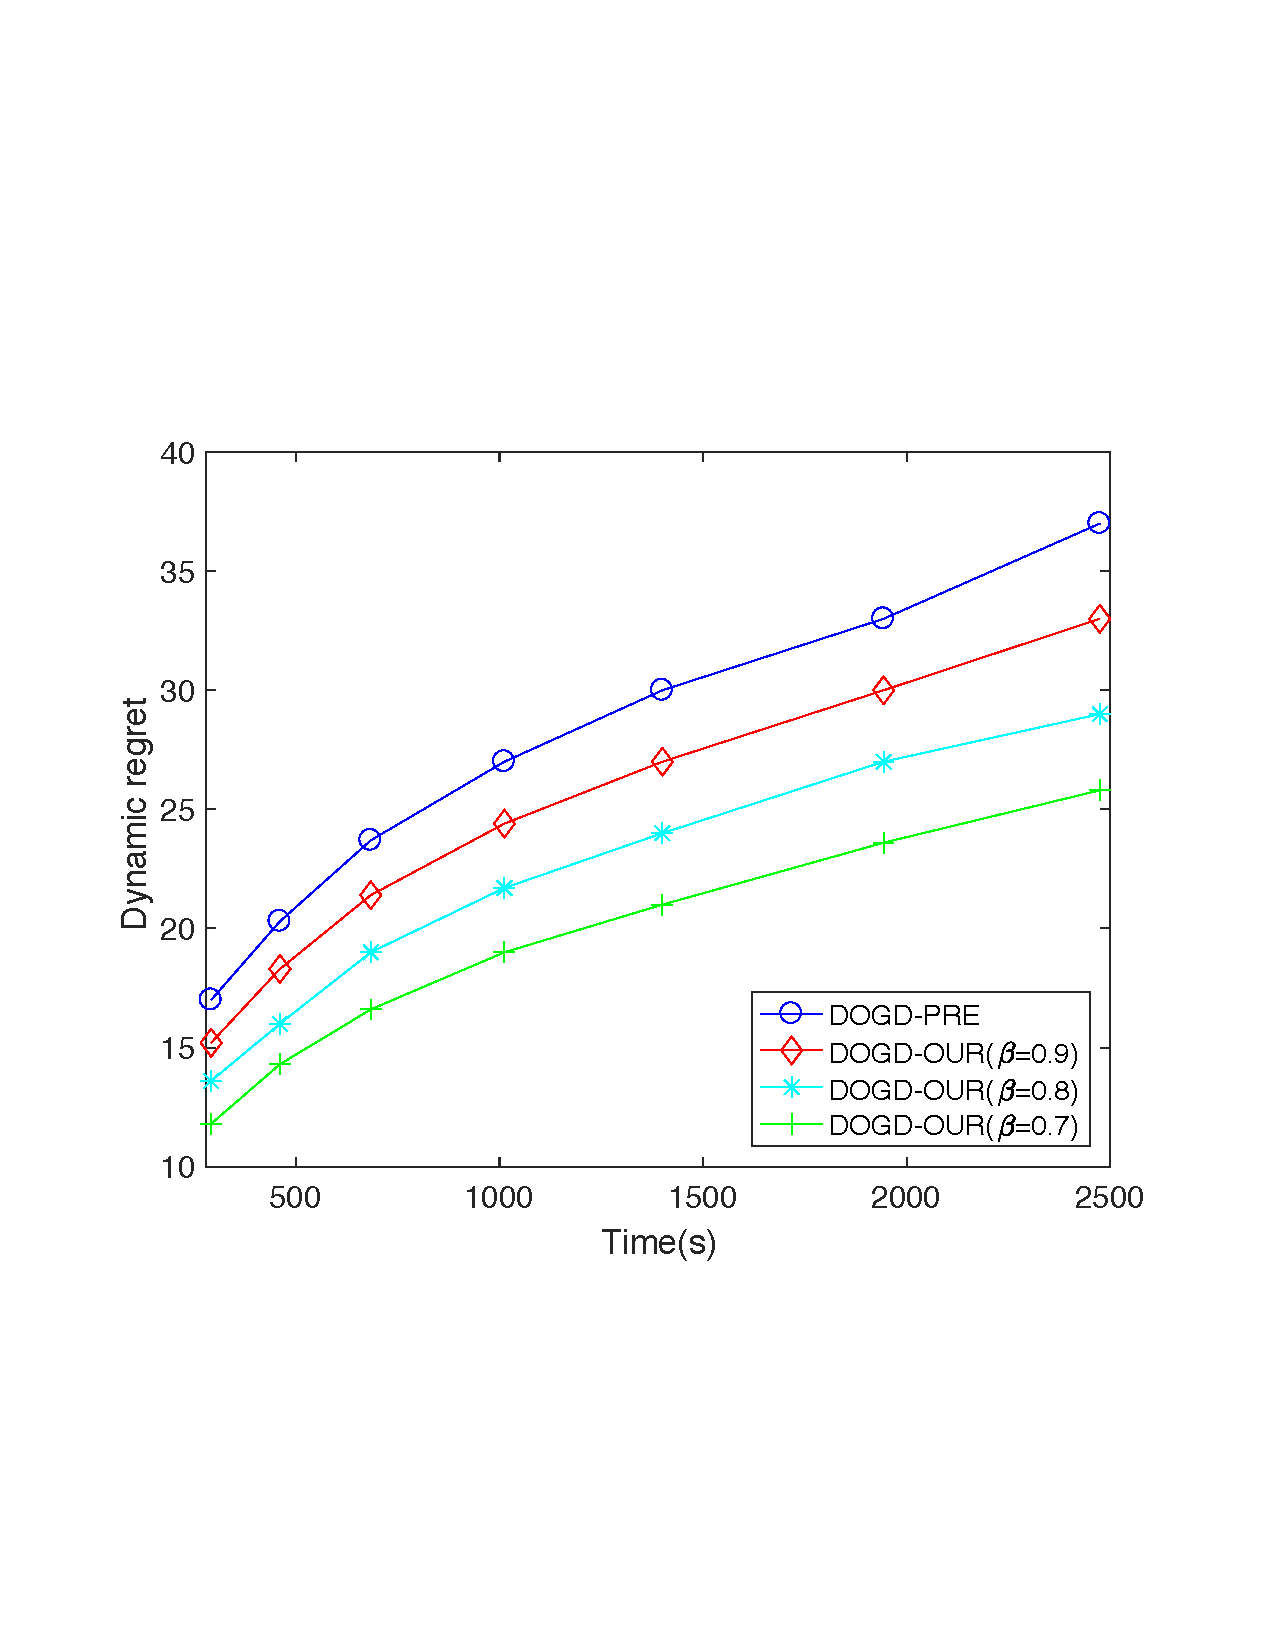
\includegraphics[width=0.45\columnwidth]{figure_regret_occupancy}\label{figure_regret_occupancy}}
\subfigure[\textit{online-retail}]{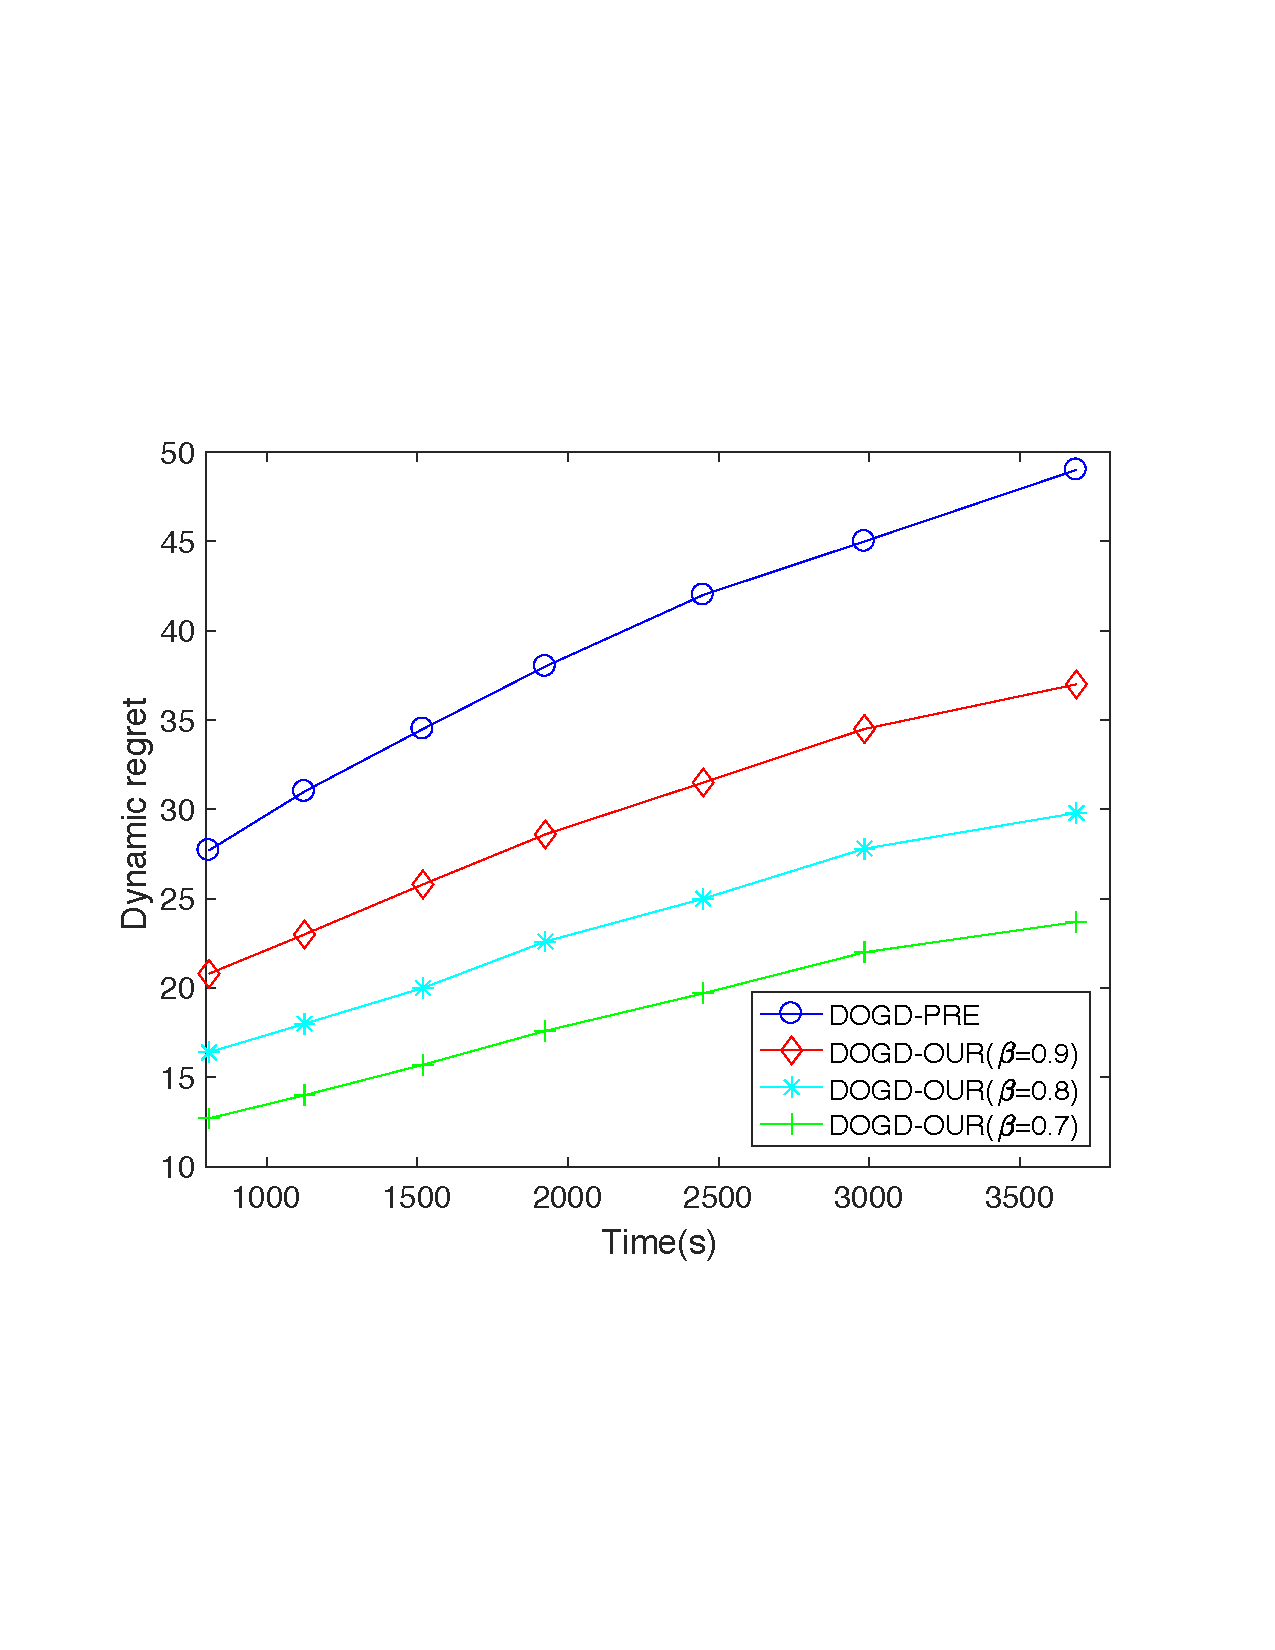
\includegraphics[width=0.45\columnwidth]{figure_regret_online-tail}\label{figure_regret_online-tail}}
\subfigure[\textit{BeijingPM2.5}]{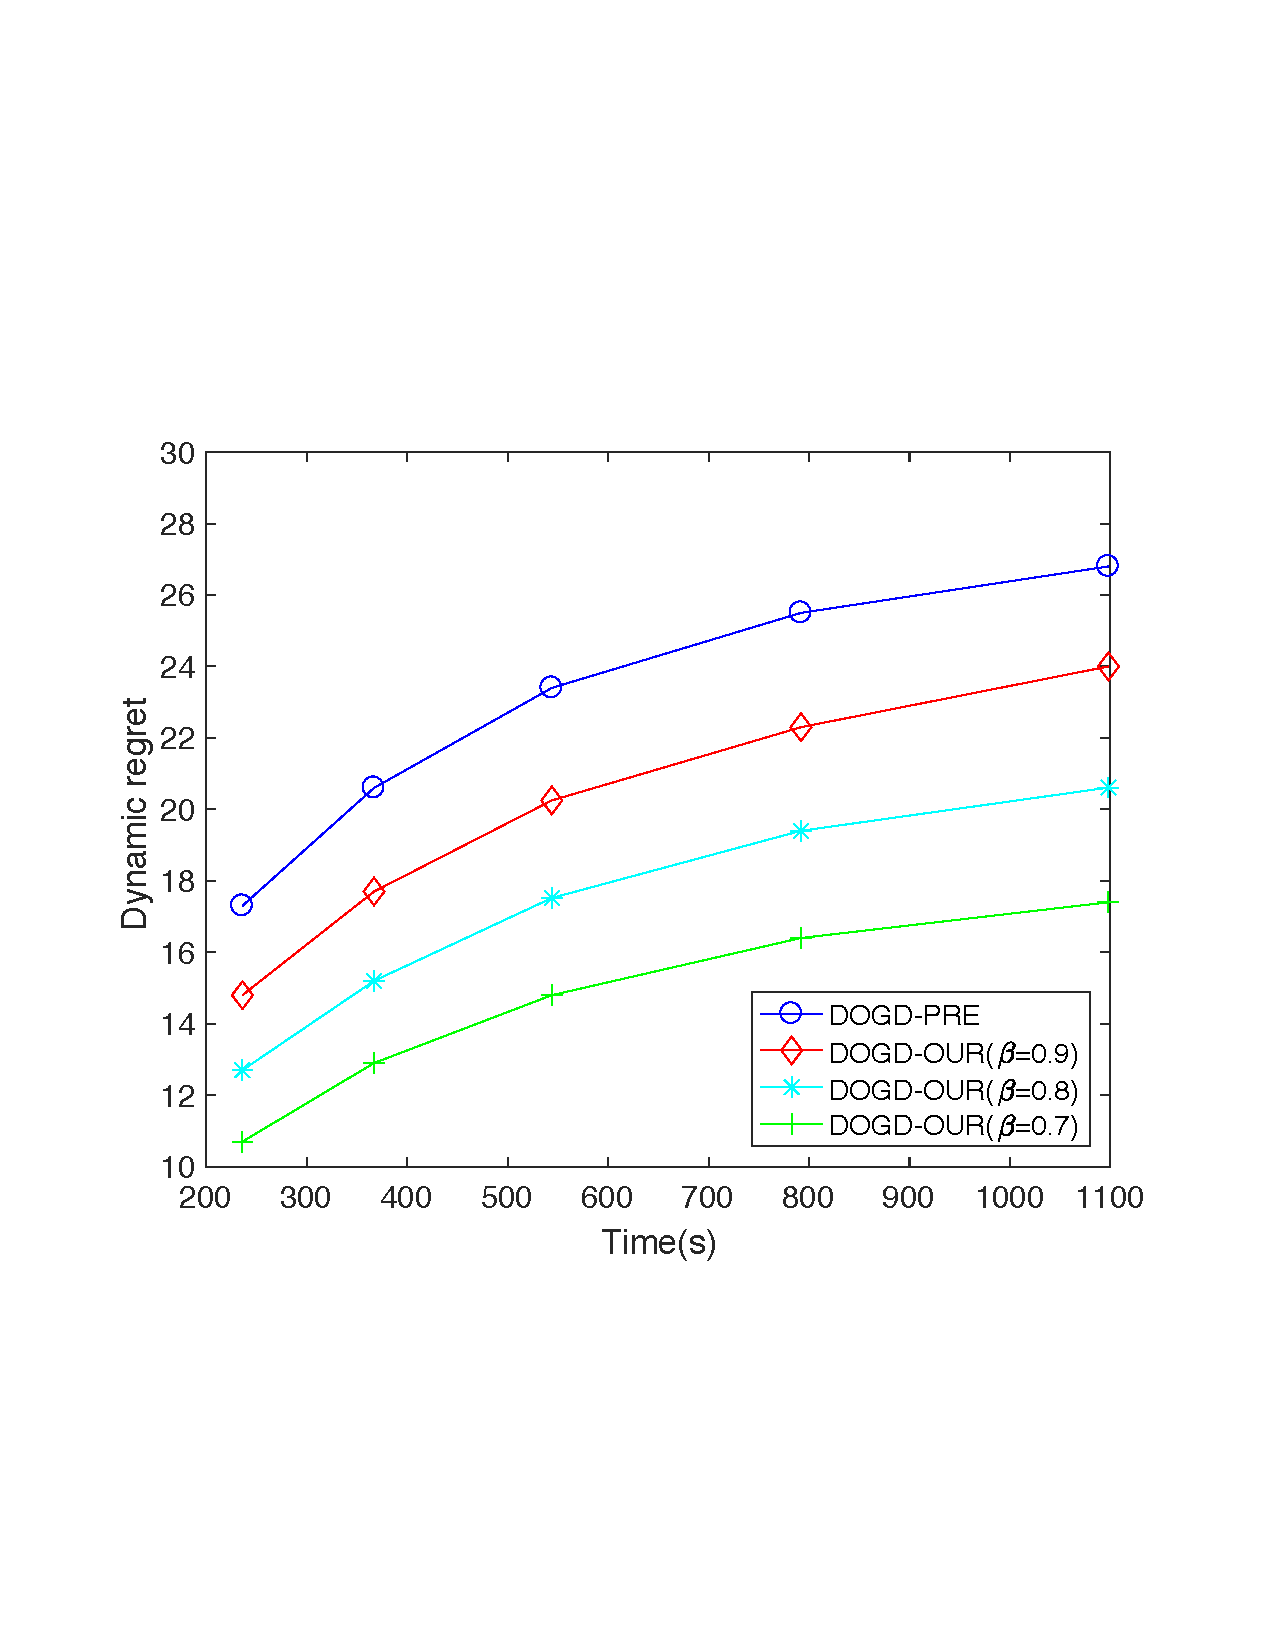
\includegraphics[width=0.45\columnwidth]{figure_regret_pm25}\label{figure_regret_pm25}}
\subfigure[\textit{spam}]{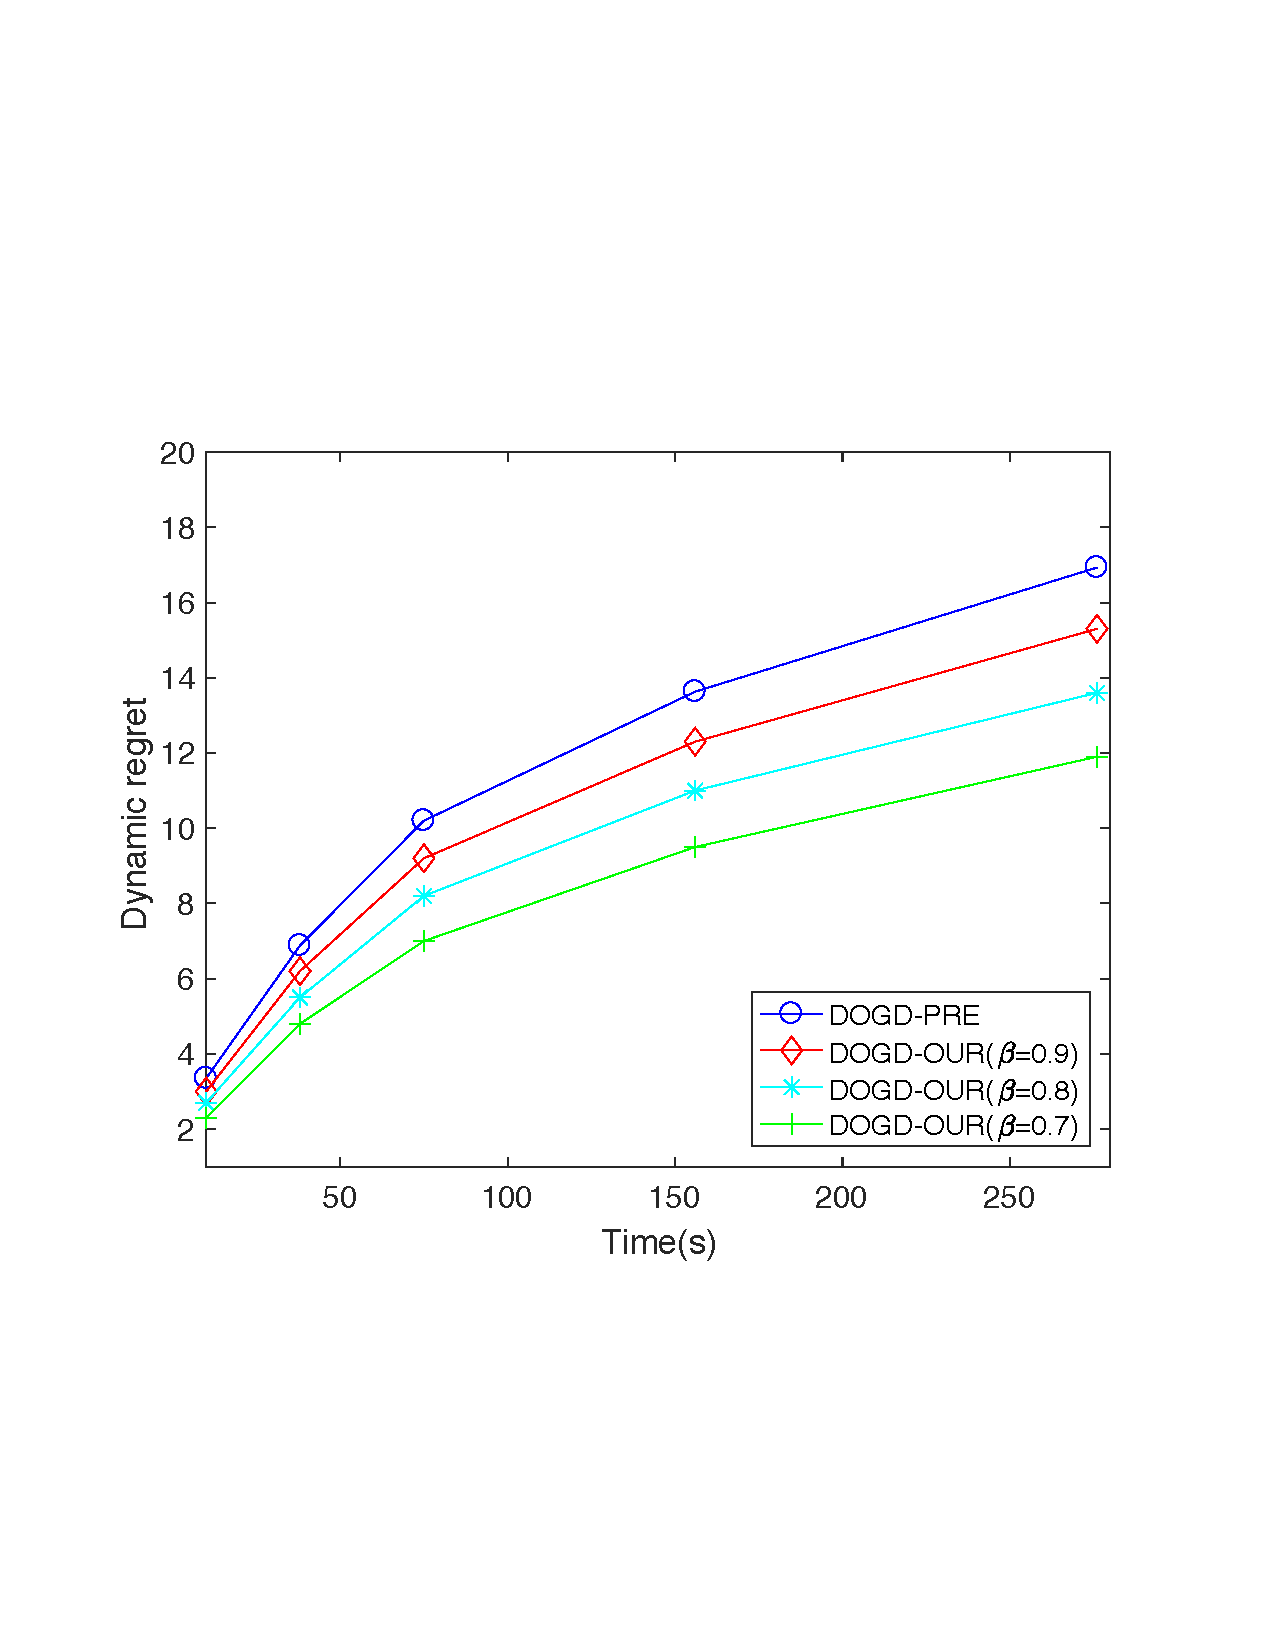
\includegraphics[width=0.45\columnwidth]{figure_regret_spam}\label{figure_regret_spam}}
\caption{Comparsion of the dynamic regret by using communication efficient logistic regression in the decentralized network.}
\label{figure_regret_communication_efficiency}
\end{figure*}





\subsection{ Online logistic regression with privacy protection}











\subsection{Online logistic regression with unrealiable features}













%\section*{References}
\bibliography{reference}

\bibliographystyle{abbrvnat}




\newpage



\section*{Appendix}

\textbf{Proof to Theorem \ref{theorem_regret_upper_bound}:}
\begin{proof}
\begin{align}
\nonumber
& \EE_{ \Xi_{n,t} \sim \Dcal_{n,t} } \frac{1}{n}\sum_{i=1}^n f_{i,t}(\x_{i,t};\xi_{i,t}) - f_{i,t}(\x_t^\ast;\xi_{i,t}) \\ \nonumber
\le & \EE_{ \Xi_{n,t} \sim \Dcal_{n,t} } \frac{1}{n}\sum_{i=1}^n \lrangle{ \partial f_{i,t}(\x_{i,t};\xi_{i,t}),  \x_{i,t} - \x_t^\ast } \\ \nonumber
= & \EE_{ \Xi_{n,t} \sim \Dcal_{n,t} }\frac{1}{n}\sum_{i=1}^n \beta \lrangle{\partial g_{i,t}(\x_{i,t}), \x_{i,t} - \x_t^\ast } + (1-\beta) \EE_{ \Xi_{n,t} \sim \Dcal_{n,t} } \frac{1}{n}\sum_{i=1}^n \lrangle{\nabla h_t(\x_{i,t};\xi_{i,t}), \x_{i,t} - \x_t^\ast } \\ \nonumber
 = & \EE_{ \Xi_{n,t} \sim \Dcal_{n,t} }\frac{1}{n}\sum_{i=1}^n \beta \lrincir{\lrangle{\partial g_{i,t}(\x_{i,t}), \x_{i,t} - \bar{\x}_t } + \lrangle{\partial g_{i,t}(\x_{i,t}), \bar{\x}_t - \bar{\x}_{t+1}} + \lrangle{\partial g_{i,t}(\x_{i,t}), \bar{\x}_{t+1} - \x_t^\ast  } } \\ \nonumber 
 & + \frac{1}{n}\EE_{ \Xi_{n,t} \sim \Dcal_{n,t} }\sum_{i=1}^n (1-\beta) \lrincir{  \lrangle{\nabla h_t(\x_{i,t};\xi_{i,t}), \x_{i,t} - \bar{\x}_t } +  \lrangle{\nabla h_t(\x_{i,t};\xi_{i,t}), \bar{\x}_t - \bar{\x}_{t+1} } } \\ \nonumber 
 & + \frac{1}{n}\EE_{ \Xi_{n,t} \sim \Dcal_{n,t} }\sum_{i=1}^n (1-\beta) \lrincir{ \lrangle{\nabla h_t(\x_{i,t};\xi_{i,t}), \bar{\x}_{t+1} - \x_t^\ast } }\\ \nonumber
= & \underbrace{ \EE_{ \Xi_{n,t} \sim \Dcal_{n,t} } \frac{1}{n}\sum_{i=1}^n \beta \lrincir{\lrangle{\partial g_{i,t}(\x_{i,t}), \x_{i,t} - \bar{\x}_t } + \lrangle{\partial g_{i,t}(\x_{i,t}), \bar{\x}_t - \bar{\x}_{t+1} } } }_{I_1(t)} \\ \nonumber 
 & + \underbrace{ \EE_{ \Xi_{n,t} \sim \Dcal_{n,t} } \frac{1}{n}\sum_{i=1}^n (1-\beta) \lrincir{ \lrangle{\nabla h_t(\x_{i,t}; \xi_{i,t}), \x_{i,t} - \bar{\x}_t } +   \lrangle{\nabla h_t(\x_{i,t};\xi_{i,t}), \bar{\x}_t - \bar{\x}_{t+1} }} }_{I_2(t)}\\ \nonumber 
&+ \underbrace{ \EE_{ \Xi_{n,t} \sim \Dcal_{n,t} } \lrangle{\frac{1}{n}\sum_{i=1}^n\partial f_{i,t}(\x_{i,t};\xi_{i,t}), \bar{\x}_{t+1} - \x_t^\ast } }_{I_3(t)}\\ \nonumber
\end{align}

Now, we begin to bound $I_1(t)$.
\begin{align}
\nonumber
I_1(t) \refabovecir{\le}{\textcircled{1}} & \EE_{ \Xi_{n,t} \sim \Dcal_{n,t} }\frac{\beta}{n}\sum_{i=1}^n \lrincir{ \frac{\eta}{2}\lrnorm{\partial g_{i,t}(\x_{i,t})}^2 + \frac{1}{2\eta}\lrnorm{\x_{i,t} - \bar{\x}_t}^2  + \frac{\eta}{2}\lrnorm{\partial g_{i,t}(\x_{i,t})}^2 + \frac{1}{2\eta}\lrnorm{\bar{\x}_t - \bar{\x}_{t+1}}^2 }\\ \nonumber
\le & \beta G \eta + \frac{\beta}{2n\eta } \EE_{ \Xi_{n,t} \sim \Dcal_{n,t} } \sum_{i=1}^n \lrnorm{\x_{i,t} - \bar{\x}_t}^2 + \frac{\beta }{2\eta }\EE_{ \Xi_{n,t} \sim \Dcal_{n,t} } \lrnorm{\bar{\x}_t - \bar{\x}_{t+1}}^2.
\end{align} $\textcircled{1}$ holds due to $\lrangle{\a,\b} \le \frac{\eta}{2}\lrnorm{\a}^2 + \frac{1}{2\eta}\lrnorm{\b}^2$ holds for any $\eta>0$. 

Now, we begin to bound $I_2(t)$.
\begin{align}
\nonumber
I_2(t) = & (1-\beta)  \lrincir{\underbrace{ \EE_{ \Xi_{n,t} \sim \Dcal_{n,t} }\frac{1}{n}\sum_{i=1}^n\lrangle{\nabla h_t(\x_{i,t}; \xi_{i,t}), \x_{i,t} - \bar{\x}_t } }_{J_1(t)} +  \underbrace{ \EE_{ \Xi_{n,t} \sim \Dcal_{n,t} }\lrangle{\frac{1}{n}\sum_{i=1}^n \nabla h_t(\x_{i,t};\xi_{i,t}), \bar{\x}_t - \bar{\x}_{t+1} }}_{J_2(t)}}.
\end{align} For $J_1(t)$, we have
\begin{align}
\nonumber
& J_1(t) \\ \nonumber 
= & \frac{1}{n}\EE_{ \Xi_{n,t} \sim \Dcal_{n,t} }\sum_{i=1}^n\lrangle{\nabla h_t(\x_{i,t}; \xi_{i,t}), \x_{i,t} - \bar{\x}_t } \\ \nonumber
= & \frac{1}{n}\EE_{ \Xi_{n,t} \sim \Dcal_{n,t} } \sum_{i=1}^n\lrangle{\nabla h_t(\x_{i,t}; \xi_{i,t}) - \nabla H_t(\bar{\x}_t), \x_{i,t} - \bar{\x}_t } + \frac{1}{n}\EE_{ \Xi_{n,t-1} \sim \Dcal_{n,t-1} }\sum_{i=1}^n\lrangle{\nabla H_t(\bar{\x}_t), \x_{i,t} - \bar{\x}_t } \\ \nonumber
= & \frac{1}{n}\EE_{ \Xi_{n,t-1} \sim \Dcal_{n,t-1} }\sum_{i=1}^n\lrangle{\nabla H_t(\x_{i,t}) - \nabla H_t(\bar{\x}_t), \x_{i,t} - \bar{\x}_t } + \frac{1}{n}\EE_{ \Xi_{n,t-1} \sim \Dcal_{n,t-1} }\sum_{i=1}^n\lrangle{\nabla H_t(\bar{\x}_t), \x_{i,t} - \bar{\x}_t } \\ \nonumber
\refabovecir{\le}{\textcircled{1}} & \frac{L}{n}\EE_{ \Xi_{n,t-1} \sim \Dcal_{n,t-1} }\sum_{i=1}^n \lrnorm{\x_{i,t} - \bar{\x}_t}^2 + \frac{1}{n}\EE_{ \Xi_{n,t-1} \sim \Dcal_{n,t-1} }\sum_{i=1}^n\lrangle{\nabla H_t(\bar{\x}_t), \x_{i,t} - \bar{\x}_t } \\ \nonumber
\refabovecir{\le}{\textcircled{2}} & \frac{L}{n}\EE_{ \Xi_{n,t-1} \sim \Dcal_{n,t-1} }\sum_{i=1}^n \lrnorm{\x_{i,t} - \bar{\x}_t}^2 + \frac{1}{n}\EE_{ \Xi_{n,t-1} \sim \Dcal_{n,t-1} }\sum_{i=1}^n\lrincir{\frac{\eta}{2\nu}\lrnorm{\nabla H_t(\bar{\x}_t)}^2 + \frac{\nu}{2\eta}\lrnorm{\x_{i,t} - \bar{\x}_t }^2 } \\ \label{equa_theorem_temp0}
\le & \frac{L}{n}\EE_{ \Xi_{n,t-1} \sim \Dcal_{n,t-1} }\sum_{i=1}^n \lrnorm{\x_{i,t} - \bar{\x}_t}^2 + \frac{\eta}{2\nu}\EE_{ \Xi_{n,t-1} \sim \Dcal_{n,t-1} }\lrnorm{\nabla H_t(\bar{\x}_t)}^2 + \frac{\nu}{2\eta n}\EE_{ \Xi_{n,t-1} \sim \Dcal_{n,t-1} }\sum_{i=1}^n\lrnorm{\x_{i,t} - \bar{\x}_t }^2. 
\end{align} $\textcircled{1}$ holds due to $H_t$ has $L$-Lipschitz gradients. $\textcircled{2}$ holds because that $\lrangle{\a,\b} \le \frac{\nu}{2}\lrnorm{\a}^2 + \frac{1}{2\nu}\lrnorm{\b}^2$ holds for any $\nu>0$. 


For $J_2(t)$, we have
\begin{align}
\nonumber
& J_2(t) \\ \nonumber 
= & \EE_{ \Xi_{n,t} \sim \Dcal_{n,t} }\lrangle{\frac{1}{n}\sum_{i=1}^n\nabla h_t(\x_{i,t};\xi_{i,t}), \bar{\x}_t - \bar{\x}_{t+1} } \\ \nonumber
\le & \frac{\eta}{2}\EE_{ \Xi_{n,t} \sim \Dcal_{n,t} } \lrnorm{\frac{1}{n}\sum_{i=1}^n \nabla h_t(\x_{i,t};\xi_{i,t})}^2 + \frac{1}{2\eta} \EE_{ \Xi_{n,t} \sim \Dcal_{n,t} }\lrnorm{ \bar{\x}_t - \bar{\x}_{t+1}}^2  \\ \nonumber
\le & \frac{\eta}{2}\EE_{ \Xi_{n,t} \sim \Dcal_{n,t} }\lrnorm{\frac{1}{n}\sum_{i=1}^n \lrincir{\nabla  h_t(\x_{i,t};\xi_{i,t}) - \nabla H_t(\x_{i,t}) + \nabla H_t(\x_{i,t})} }^2 + \frac{1}{2\eta} \EE_{ \Xi_{n,t} \sim \Dcal_{n,t} }\lrnorm{ \bar{\x}_t - \bar{\x}_{t+1}}^2  \\ \nonumber
\le &  \eta\EE_{ \Xi_{n,t} \sim \Dcal_{n,t} }\lrnorm{\frac{1}{n}\sum_{i=1}^n \lrincir{ \nabla h_t(\x_{i,t};\xi_{i,t}) - \nabla H_t(\x_{i,t}) } }^2 + \eta \EE_{ \Xi_{n,t-1} \sim \Dcal_{n,t-1} }\lrnorm{\frac{1}{n}\sum_{i=1}^n\nabla H_t(\x_{i,t})}^2 \\ \nonumber 
& + \frac{1}{2\eta} \EE_{ \Xi_{n,t} \sim \Dcal_{n,t} }\lrnorm{ \bar{\x}_t - \bar{\x}_{t+1}}^2  \\ \nonumber
\refabovecir{\le}{\textcircled{1}} & \frac{\eta}{n} \sigma^2 + \eta \EE_{ \Xi_{n,t-1} \sim \Dcal_{n,t-1} }\lrnorm{ \frac{1}{n}\sum_{i=1}^n \lrincir{ \nabla H_t(\x_{i,t}) - \nabla H_t(\bar{\x}_t) + \nabla H_t(\bar{\x}_t) } }^2 + \frac{1}{2\eta} \EE_{ \Xi_{n,t} \sim \Dcal_{n,t} }\lrnorm{ \bar{\x}_t - \bar{\x}_{t+1}}^2 \\ \nonumber
\le & \frac{\eta}{n} \sigma^2 + 2\eta \EE_{ \Xi_{n,t-1} \sim \Dcal_{n,t-1} }\lrnorm{\frac{1}{n}\sum_{i=1}^n \lrincir{ \nabla H_t(\x_{i,t}) - \nabla H_t(\bar{\x}_t) } }^2 \\ \nonumber 
& + 2\eta \EE_{ \Xi_{n,t-1} \sim \Dcal_{n,t-1} }\lrnorm{\nabla H_t(\bar{\x}_t)}^2 + \frac{1}{2\eta} \EE_{ \Xi_{n,t} \sim \Dcal_{n,t} }\lrnorm{ \bar{\x}_t - \bar{\x}_{t+1}}^2 \\ \nonumber
\le & \frac{\eta}{n} \sigma^2 + \frac{2\eta}{n} \EE_{ \Xi_{n,t-1} \sim \Dcal_{n,t-1} }\sum_{i=1}^n\lrnorm{ \nabla H_t(\x_{i,t}) - \nabla H_t(\bar{\x}_t)  }^2 \\ \nonumber 
& + 2\eta \EE_{ \Xi_{n,t-1} \sim \Dcal_{n,t-1} }\lrnorm{\nabla H_t(\bar{\x}_t)}^2 + \frac{1}{2\eta} \EE_{ \Xi_{n,t} \sim \Dcal_{n,t} }\lrnorm{ \bar{\x}_t - \bar{\x}_{t+1}}^2 \\ \nonumber
\refabovecir{\le}{\textcircled{2}} & \frac{\eta}{n} \sigma^2 + \frac{2\eta L^2}{n}\EE_{ \Xi_{n,t-1} \sim \Dcal_{n,t-1} }\sum_{i=1}^n \lrnorm{\x_{i,t} - \bar{\x}_t }^2 + 2\eta \EE_{ \Xi_{n,t-1} \sim \Dcal_{n,t-1} }\lrnorm{\nabla H_t(\bar{\x}_t)}^2 + \frac{1}{2\eta} \EE_{ \Xi_{n,t} \sim \Dcal_{n,t} }\lrnorm{ \bar{\x}_t - \bar{\x}_{t+1}}^2.
\end{align} $\textcircled{1}$ holds due to
\begin{align}
\nonumber
& \EE_{ \Xi_{n,t} \sim \Dcal_{n,t} }\lrnorm{\frac{1}{n}\sum_{i=1}^n \lrincir{ \nabla h_t(\x_{i,t};\xi_{i,t}) - \nabla H_t(\x_{i,t}) } }^2 \\ \nonumber
= & \frac{1}{n^2}\EE_{ \Xi_{n,t-1} \sim \Dcal_{n,t-1} }\lrincir{ \sum_{i=1}^n \EE_{ \xi_{i,t} \sim D_{i,t} }\lrnorm{ \nabla h_t(\x_{i,t};\xi_{i,t}) - \nabla H_t(\x_{i,t}) }^2  } \\ \nonumber 
& + \frac{1}{n^2}\EE_{ \Xi_{n,t-1} \sim \Dcal_{n,t-1} }\lrincir{2\sum_{i=1}^n\sum_{j=1, j\neq i}^n\lrangle{ \EE_{ \xi_{i,t} \sim D_{i,t} }\nabla h_t(\x_{i,t};\xi_{i,t}) - \nabla H_t(\x_{i,t}),  \EE_{ \xi_{j,t} \sim D_{j,t} } \nabla h_t(\x_{j,t};\xi_{j,t}) - \nabla H_t(\x_{j,t})} } \\ \nonumber
= & \frac{1}{n^2}\EE_{ \Xi_{n,t-1} \sim \Dcal_{n,t-1} }\sum_{i=1}^n \EE_{ \xi_{i,t} \sim D_{i,t} }\lrnorm{ \nabla h_t(\x_{i,t};\xi_{i,t}) - \nabla H_t(\x_{i,t}) }^2 + 0 \\ \nonumber
\le & \frac{1}{n} \sigma^2.
\end{align} $\textcircled{2}$ holds due to $H_t$ has $L$ Lipschitz gradients.

 Therefore, we obtain
\begin{align}
\nonumber
& I_2(t) \\ \nonumber 
= & (1-\beta)(J_1(t) + J_2(t)) \\ \nonumber
= &  (1-\beta)\lrincir{ \frac{L}{n}\EE_{ \Xi_{n,t-1} \sim \Dcal_{n,t-1} }\sum_{i=1}^n \lrnorm{\x_{i,t} - \bar{\x}_t}^2 + \frac{\eta}{2\nu}\EE_{ \Xi_{n,t-1} \sim \Dcal_{n,t-1} }\lrnorm{\nabla H_t(\bar{\x}_t)}^2 + \frac{\nu}{2\eta n}\EE_{ \Xi_{n,t-1} \sim \Dcal_{n,t-1} }\sum_{i=1}^n\lrnorm{\x_{i,t} - \bar{\x}_t }^2 } \\ \nonumber
& + (1-\beta)\lrincir{ \frac{\eta}{n} \sigma^2 + \frac{2\eta L^2}{n}\EE_{ \Xi_{n,t-1} \sim \Dcal_{n,t-1} }\sum_{i=1}^n \lrnorm{\x_{i,t} - \bar{\x}_t }^2 } \\ \nonumber 
& + (1-\beta)\lrincir{ 2\eta \EE_{ \Xi_{n,t-1} \sim \Dcal_{n,t-1} }\lrnorm{\nabla H_t(\bar{\x}_t)}^2 + \frac{1}{2\eta} \EE_{ \Xi_{n,t} \sim \Dcal_{n,t} }\lrnorm{ \bar{\x}_t - \bar{\x}_{t+1}}^2 } \\ \nonumber
\le &  (1-\beta)\lrincir{ \frac{L}{n} + \frac{\nu}{2n\eta} + \frac{2\eta L^2}{n} }\EE_{ \Xi_{n,t-1} \sim \Dcal_{n,t-1} }\sum_{i=1}^n\lrnorm{\x_{i,t} - \bar{\x}_t }^2   + \lrincir{ \frac{\eta}{2\nu} + 2\eta }(1-\beta)\EE_{ \Xi_{n,t-1} \sim \Dcal_{n,t-1} }\lrnorm{\nabla H_t(\bar{\x}_t)}^2 \\ \nonumber 
&+ \frac{\eta (1-\beta)\sigma^2}{n} +  \frac{1-\beta}{2\eta} \EE_{ \Xi_{n,t} \sim \Dcal_{n,t} }\lrnorm{ \bar{\x}_t - \bar{\x}_{t+1}}^2.
\end{align}

Combine those bounds of $I_1(t)$ and $I_2(t)$. We thus have
\begin{align}
\nonumber
& I_1(t) + I_2(t) \\ \nonumber 
\le & \beta G \eta + \frac{\beta}{2n\eta }\sum_{i=1}^n \EE_{ \Xi_{n,t-1} \sim \Dcal_{n,t-1} }\lrnorm{\x_{i,t} - \bar{\x}_t}^2 + \frac{\beta }{2\eta } \EE_{ \Xi_{n,t} \sim \Dcal_{n,t} }\lrnorm{\bar{\x}_t - \bar{\x}_{t+1}}^2 \\ \nonumber
& + (1-\beta)\lrincir{ \frac{L}{n} + \frac{\nu}{2n\eta} + \frac{2\eta L^2}{n} }\EE_{ \Xi_{n,t-1} \sim \Dcal_{n,t-1} }\sum_{i=1}^n\lrnorm{\x_{i,t} - \bar{\x}_t }^2   + \lrincir{ \frac{\eta}{2\nu} + 2\eta }(1-\beta)\EE_{ \Xi_{n,t-1} \sim \Dcal_{n,t-1} }\lrnorm{\nabla H_t(\bar{\x}_t)}^2 \\ \nonumber 
&+ \frac{\eta (1-\beta)\sigma^2}{n} +  \frac{1-\beta}{2\eta} \EE_{ \Xi_{n,t} \sim \Dcal_{n,t} }\lrnorm{ \bar{\x}_t - \bar{\x}_{t+1}}^2 \\ \nonumber
= & \eta\lrincir{ \beta G + \frac{(1-\beta)\sigma^2}{n}} + (1-\beta)\lrincir{\frac{\beta}{2n\eta } +\frac{L}{n} + \frac{\nu}{2n\eta} + \frac{2\eta L^2}{n} }\sum_{i=1}^n \EE_{ \Xi_{n,t-1} \sim \Dcal_{n,t-1} }\lrnorm{\x_{i,t} - \bar{\x}_t}^2 \\ \nonumber
& + \frac{1}{2\eta } \EE_{ \Xi_{n,t} \sim \Dcal_{n,t} }\lrnorm{\bar{\x}_t - \bar{\x}_{t+1}}^2  + \lrincir{ \frac{\eta}{2\nu} + 2\eta }(1-\beta)\EE_{ \Xi_{n,t-1} \sim \Dcal_{n,t-1} }\lrnorm{\nabla H_t(\bar{\x}_t)}^2. 
\end{align}

Therefore, we have 
\begin{align}
\nonumber
&\sum_{t=1}^T (I_1(t) + I_2(t)) \\ \nonumber
\le & \eta T \lrincir{ \beta G + \frac{(1-\beta)\sigma^2}{n}} + (1-\beta)\lrincir{\frac{\beta}{2n\eta } +\frac{L}{n} + \frac{\nu}{2n\eta} + \frac{2\eta L^2}{n} } \EE_{ \Xi_{n,T-1} \sim \Dcal_{n,T-1} }\sum_{i=1}^n \sum_{t=1}^T \lrnorm{\x_{i,t} - \bar{\x}_t}^2  \\ \nonumber
& + \frac{1}{2\eta } \EE_{ \Xi_{n,T} \sim \Dcal_{n,T} }\sum_{t=1}^T \lrnorm{\bar{\x}_t - \bar{\x}_{t+1}}^2 + \lrincir{ \frac{\eta}{2\nu} + 2\eta }(1-\beta)\EE_{ \Xi_{n,T-1} \sim \Dcal_{n,T-1} }\sum_{t=1}^T\lrnorm{\nabla H_t(\bar{\x}_t)}^2.
\end{align} 




Now, we begin to bound $I_3(t)$. Recall that the update rule is 
\begin{align}
\nonumber
\x_{i,t+1} = \sum_{j=1}^n \W_{ij}\x_{j,t} - \eta \partial f_{i,t}(\x_{i,t};\xi_{i,t}).
\end{align}  According to Lemma \ref{lemma_average_update_rule}, we have 
\begin{align}
\label{equa_thoerem_update_rule_equivalent}
\bar{\x}_{t+1} = \bar{\x}_t - \eta \lrincir{\frac{1}{n}\sum_{i=1}^n \partial f_{i,t}(\x_{i,t};\xi_{i,t})}.
\end{align} 
Denote a new auxiliary function $\phi(\z)$ as 
\begin{align}
\nonumber
\phi(\z) = \lrangle{\frac{1}{n}\sum_{i=1}^n \partial f_{i,t}(\x_{i,t};\xi_{i,t}), \z} + \frac{1}{2\eta}\lrnorm{\z - \bar{\x}_t}^2.
\end{align} 

It is trivial to verify that \eqref{equa_thoerem_update_rule_equivalent} satisfies the first-order optimality condition of the optimization problem: $\min_{\z\in\RR^d} \phi(\z)$, that is,
\begin{align}
\nonumber
\nabla \phi(\bar{\x}_{t+1}) = \0.
\end{align} We thus have 
\begin{align}
\nonumber
\bar{\x}_{t+1} = & \argmin_{\z\in\RR^d} \phi(\z) \\ \nonumber
= & \argmin_{\z\in\RR^d} \lrangle{\frac{1}{n}\sum_{i=1}^n \partial f_{i,t}(\x_{i,t};\xi_{i,t}), \z} + \frac{1}{2\eta}\lrnorm{\z - \bar{\x}_t}^2.
\end{align} Furthermore, denote a new auxiliary variable $\bar{\x}_{\tau}$ as  
\begin{align}
\nonumber
\bar{\x}_{\tau} = \bar{\x}_{t+1} + \tau \lrincir{\x_t^\ast - \bar{\x}_{t+1}},
\end{align} where $0< \tau \le 1$. According to the optimality of $\bar{\x}_{t+1}$, we have
\begin{align}
\nonumber
0 \le & \phi(\bar{\x}_{\tau}) - \phi(\bar{\x}_{t+1}) \\ \nonumber
= & \lrangle{\frac{1}{n}\sum_{i=1}^n \partial f_{i,t}(\x_{i,t};\xi_{i,t}), \bar{\x}_{\tau} - \bar{\x}_{t+1}} + \frac{1}{2\eta}\lrincir{ \lrnorm{\bar{\x}_{\tau} - \bar{\x}_t}^2 - \lrnorm{\bar{\x}_{t+1} - \bar{\x}_t}^2 } \\ \nonumber
= & \lrangle{\frac{1}{n}\sum_{i=1}^n \partial f_{i,t}(\x_{i,t};\xi_{i,t}), \tau \lrincir{\x_t^\ast - \bar{\x}_{t+1}}} + \frac{1}{2\eta}\lrincir{ \lrnorm{\bar{\x}_{t+1} + \tau \lrincir{\x_t^\ast - \bar{\x}_{t+1}} - \bar{\x}_t}^2 - \lrnorm{\bar{\x}_{t+1} - \bar{\x}_t}^2 } \\ \nonumber
= & \lrangle{\frac{1}{n}\sum_{i=1}^n \partial f_{i,t}(\x_{i,t};\xi_{i,t}), \tau \lrincir{\x_t^\ast - \bar{\x}_{t+1}}} + \frac{1}{2\eta}\lrincir{ \lrnorm{\tau \lrincir{\x_t^\ast - \bar{\x}_{t+1}}}^2 + 2\lrangle{\tau \lrincir{\x_t^\ast - \bar{\x}_{t+1}}, \bar{\x}_{t+1} - \bar{\x}_t } }.
\end{align} Note that the above inequality holds for any $0< \tau \le 1$. Divide $\tau$ on both sides, and we have
\begin{align}
\nonumber
I_3(t) = & \EE_{ \Xi_{n,t} \sim \Dcal_{n,t} } \lrangle{\frac{1}{n}\sum_{i=1}^n \partial f_{i,t}(\x_{i,t};\xi_{i,t}), \bar{\x}_{t+1} - \x_t^\ast} \\ \nonumber 
\le & \frac{1}{2\eta}\EE_{ \Xi_{n,t} \sim \Dcal_{n,t} }\lrincir{ \lim_{\tau \rightarrow 0^+}\tau \lrnorm{\lrincir{\x_t^\ast - \bar{\x}_{t+1}}}^2 + 2\lrangle{ \x_t^\ast - \bar{\x}_{t+1}, \bar{\x}_{t+1} - \bar{\x}_t } } \\ \nonumber
= & \frac{1}{\eta}\EE_{ \Xi_{n,t} \sim \Dcal_{n,t} }\lrangle{ \x_t^\ast - \bar{\x}_{t+1}, \bar{\x}_{t+1} - \bar{\x}_t } \\ \label{equa_I3_temp}
= & \frac{1}{2\eta}\EE_{ \Xi_{n,t} \sim \Dcal_{n,t} }\lrincir{ \lrnorm{\x_t^\ast - \bar{\x}_t}^2 - \lrnorm{\x_t^\ast - \bar{\x}_{t+1}}^2 - \lrnorm{\bar{\x}_t - \bar{\x}_{t+1}}^2 }. 
\end{align} Besides, we have
\begin{align}
\nonumber
& \lrnorm{\x_{t+1}^\ast - \bar{\x}_{t+1}}^2 - \lrnorm{\x_t^\ast - \bar{\x}_{t+1}}^2 \\ \nonumber 
= & \lrnorm{\x_{t+1}^\ast}^2 - \lrnorm{\x_t^\ast}^2 - 2\lrangle{\bar{\x}_{t+1}, -\x_t^\ast + \x_{t+1}^\ast} \\ \nonumber
= & \lrincir{\lrnorm{\x_{t+1}^\ast} - \lrnorm{\x_t^\ast}} \lrincir{\lrnorm{\x_{t+1}^\ast} + \lrnorm{\x_t^\ast}} - 2\lrangle{\bar{\x}_{t+1}, -\x_t^\ast + \x_{t+1}^\ast} \\ \nonumber
\le & \lrnorm{\x_{t+1}^\ast - \x_t^\ast} \lrincir{\lrnorm{\x_{t+1}^\ast} + \lrnorm{\x_t^\ast}} + 2\lrnorm{\bar{\x}_{t+1}} \lrnorm{\x_{t+1}^\ast-\x_t^\ast} \\ \nonumber
\le & 4\sqrt{R}\lrnorm{\x_{t+1}^\ast - \x_t^\ast}.   
\end{align} The last inequality holds due to our assumption, that is, $\lrnorm{\x_{t+1}^\ast}=\lrnorm{\x_{t+1}^\ast - \0}\le \sqrt{R}$, $\lrnorm{\x_t^\ast} = \lrnorm{\x_t^\ast-\0} \le \sqrt{R}$, and $\lrnorm{\bar{\x}_{t+1}} = \lrnorm{\bar{\x}_{t+1}-\0} \le \sqrt{R}$. 

Thus, telescoping $I_3(t)$ over $t\in[T]$, we have 
\begin{align}
\nonumber
& \sum_{t=1}^T I_3(t) \\ \nonumber 
\le & \frac{1}{2\eta}\EE_{ \Xi_{n,T} \sim \Dcal_{n,T} }\lrincir{ 4\sqrt{R}\sum_{t=1}^T\lrnorm{\x_{t+1}^\ast - \x_t^\ast} + \lrnorm{\bar{\x}_1^\ast - \bar{\x}_1}^2 - \lrnorm{\bar{\x}_T^\ast - \bar{\x}_{T+1}}^2 } - \frac{1}{2\eta} \EE_{ \Xi_{n,T} \sim \Dcal_{n,T} }\sum_{t=1}^T \lrnorm{\bar{\x}_t - \bar{\x}_{t+1}}^2 \\ \nonumber
\le & \frac{1}{2\eta}\lrincir{ 4\sqrt{R} M + R } - \frac{1}{2\eta} \EE_{ \Xi_{n,T} \sim \Dcal_{n,T} } \sum_{t=1}^T \lrnorm{\bar{\x}_t - \bar{\x}_{t+1} }^2.
\end{align} Here, $M$ the budget of the dynamics, which is defined in \eqref{equa_define_M}.


Combining those bounds of $I_1(t)$, $I_2(t)$ and $I_3(t)$ together, we finally obtain
\begin{align}
\nonumber
& \EE_{ \Xi_{n,T} \sim \Dcal_{n,T} } \sum_{t=1}^T\sum_{i=1}^n f_{i,t}(\x_{i,t};\xi_{i,t}) - f_t(\x_t^\ast;\xi_{i,t}) \\ \nonumber
\le & n \sum_{t=1}^T \lrincir{ I_1(t) + I_2(t) + I_3(t) } \\ \nonumber
\le & \eta T \lrincir{ n\beta G + (1-\beta)\sigma^2} + (1-\beta)\lrincir{\frac{\beta}{2\eta } +L + \frac{\nu}{2\eta} + 2\eta L^2 } \EE_{ \Xi_{n,T} \sim \Dcal_{n,T} }\sum_{i=1}^n \sum_{t=1}^T \lrnorm{\x_{i,t} - \bar{\x}_t}^2  \\ \nonumber
& + n\lrincir{ \frac{\eta}{2\nu} + 2\eta }(1-\beta)\EE_{ \Xi_{n,T-1} \sim \Dcal_{n,T-1} }\sum_{t=1}^T\lrnorm{\nabla H_t(\bar{\x}_t)}^2  + \frac{n}{2\eta}\lrincir{ 4\sqrt{R}M + R  } \\ \nonumber
\refabovecir{\le}{\textcircled{1}} & \eta T \lrincir{ n\beta G + (1-\beta)\sigma^2} + n(1-\beta)\lrincir{ \frac{1}{\nu} + 4 } \lrincir{ \EE_{ \Xi_{n,T} \sim \Dcal_{n,T} } \sum_{t=1}^T  \lrincir{H_t(\bar{\x}_t) - H_t(\bar{\x}_{t+1})}  } \\ \nonumber
& + (1-\beta)\lrincir{\frac{\beta}{2\eta } +L + \frac{\nu}{2\eta} + 2\eta L^2  + \lrincir{\frac{1}{\nu} + 4}(1-\beta)^2L^2 \eta}  \EE_{ \Xi_{n,T} \sim \Dcal_{n,T} }\sum_{t=1}^T\sum_{i=1}^n \lrnorm{ \bar{\x}_t - \x_{i,t} }^2  \\ \nonumber
& + n(1-\beta)\lrincir{ \frac{1}{\nu} + 4 } \lrincir{ 4T\beta^2 \eta G + \frac{TGL\eta^2}{2} }  + \frac{n}{2\eta}\lrincir{ 4\sqrt{R}M + R  }\\ \nonumber
\refabovecir{\le}{\textcircled{2}} & \eta T \lrincir{ n\beta G + (1-\beta)\sigma^2} + n(1-\beta)\lrincir{ \frac{1}{\nu} + 4 } \lrincir{ \EE_{ \Xi_{n,T} \sim \Dcal_{n,T} } \sum_{t=1}^T  \lrincir{H_t(\bar{\x}_t) - H_t(\bar{\x}_{t+1})}  } \\ \nonumber
& + (1-\beta)\lrincir{\frac{\beta}{2\eta } +L + \frac{\nu}{2\eta} + 2\eta L^2  + \lrincir{\frac{1}{\nu} + 4}(1-\beta)^2L^2 \eta}  \frac{nT\eta^2 G }{(1-\rho)^2}  \\ \nonumber
& + n(1-\beta)\lrincir{ \frac{1}{\nu} + 4 } \lrincir{ 4T\beta^2 \eta G + \frac{TGL\eta^2}{2} }  + \frac{n}{2\eta}\lrincir{ 4\sqrt{R}M + R  }.
\end{align}  
$\textcircled{1}$ holds due to Lemma \ref{lemma_gradient_norm_bound}. That is, we have
\begin{align}
& \frac{\eta}{2} \EE_{ \Xi_{n,T-1} \sim \Dcal_{n,T-1} }\sum_{t=1}^T \lrnorm{\nabla H_t(\bar{\x}_t)}^2 \\ \nonumber
\le & \EE_{ \Xi_{n,T} \sim \Dcal_{n,T} } \sum_{t=1}^T  \lrincir{H_t(\bar{\x}_t) - H_t(\bar{\x}_{t+1})} + 4T\beta^2 \eta G + \frac{(1-\beta)^2L^2 \eta}{n}\EE_{ \Xi_{n,T-1} \sim \Dcal_{n,T-1} }\sum_{t=1}^T\sum_{i=1}^n \lrnorm{ \bar{\x}_t - \x_{i,t} }^2 + \frac{TGL\eta^2}{2}.
\end{align} 

$\textcircled{2}$ holds due to Lemma \ref{lemma_x_variance_norm_square}
\begin{align}
\nonumber
\EE_{ \Xi_{n,T-1} \sim \Dcal_{n,T-1} } \sum_{i=1}^n\sum_{t=1}^T \lrnorm{\x_{i,t} - \bar{\x}_t}^2 \le \frac{nT\eta^2 G }{(1-\rho)^2}.
\end{align}





Letting $\nu = \sqrt{\beta^2 + \eta}$, we have
\begin{align}
\nonumber
& \EE_{ \Xi_{n,T} \sim \Dcal_{n,T} } \sum_{t=1}^T\sum_{i=1}^n f_{i,t}(\x_{i,t};\xi_{i,t}) - f_{i,t}(\x_t^\ast;\xi_{i,t}) \\ \nonumber
\le & \eta T \lrincir{ n\beta G + (1-\beta)\sigma^2} + n(1-\beta)\lrincir{ \frac{1}{\sqrt{\beta^2 + \eta}} + 4 } \lrincir{ \EE_{ \Xi_{n,T} \sim \Dcal_{n,T} } \sum_{t=1}^T  \lrincir{H_t(\bar{\x}_t) - H_t(\bar{\x}_{t+1})}  } \\ \nonumber
& + (1-\beta)\lrincir{\frac{\beta}{2\eta } +L + \frac{\sqrt{\beta^2 + \eta}}{2\eta} + 2\eta L^2  + \lrincir{\frac{1}{\sqrt{\beta^2 + \eta}} + 4}(1-\beta)^2L^2 \eta}  \frac{nT\eta^2 G }{(1-\rho)^2}  \\ \nonumber
& + n(1-\beta)\lrincir{ \frac{1}{\sqrt{\beta^2 + \eta}} + 4 } \lrincir{ 4T\beta^2 \eta G + \frac{TGL\eta^2}{2} }  + \frac{n}{2\eta}\lrincir{ 4\sqrt{R}M + R  }.
\end{align}



It completes the proof.



\end{proof}


\begin{Lemma}
\label{lemma_stochastic_gradient_norm_bound}
Using Assumption \ref{assumption_bounded_gradient_domain}, we have
\begin{align}
\nonumber
\EE_{ \Xi_{n,t} \sim \Dcal_{n,t} }\lrnorm{ \partial f_{i,t}(\x_{i,t};\xi_{i,t})}^2 \le G.
\end{align}


\end{Lemma}
\begin{proof}

\begin{align}
\nonumber
& \EE_{ \Xi_{n,t} \sim \Dcal_{n,t} }\lrnorm{ \partial f_{i,t}(\x_{i,t};\xi_{i,t})}^2 \\ \nonumber 
= & \EE_{ \Xi_{n,t} \sim \Dcal_{n,t} }\lrnorm{ \beta \partial g_{i,t}(\x_{i,t}) + (1-\beta)\nabla h_t(\x_{i,t};\xi_{i,t})}^2 \\ \nonumber 
\le &  \beta \EE_{ \Xi_{n,t-1} \sim \Dcal_{n,t-1} }\lrnorm{ \partial g_{i,t}(\x_{i,t}) }^2 + (1-\beta) \EE_{ \Xi_{n,t} \sim \Dcal_{n,t} } \lrnorm{ \nabla h_t(\x_{i,t};\xi_{i,t}) }^2 \\ \nonumber 
\le & G.
\end{align} It completes the proof.
\end{proof}



\begin{Lemma}
\label{lemma_gradient_norm_bound}
Using Assumption \ref{assumption_bounded_gradient_domain}, and setting $\eta>0$ in Algorithm \ref{algo_DOG}, we have 
\begin{align}
& \frac{\eta}{2} \EE_{ \Xi_{n,T-1} \sim \Dcal_{n,T-1} }\sum_{t=1}^T \lrnorm{\nabla H_t(\bar{\x}_t)}^2 \\ \nonumber
\le & \EE_{ \Xi_{n,T} \sim \Dcal_{n,T} } \sum_{t=1}^T  \lrincir{H_t(\bar{\x}_t) - H_t(\bar{\x}_{t+1})} + 4T\beta^2 \eta G + \frac{(1-\beta)^2L^2 \eta}{n}\EE_{ \Xi_{n,T-1} \sim \Dcal_{n,T-1} }\sum_{t=1}^T\sum_{i=1}^n \lrnorm{ \bar{\x}_t - \x_{i,t} }^2 + \frac{TGL\eta^2}{2}.
\end{align}
\end{Lemma}
\begin{proof}

\begin{align}
\nonumber
& \EE_{ \Xi_{n,t} \sim \Dcal_{n,t} } H_t(\bar{\x}_{t+1}) \\ \nonumber
\le & \EE_{ \Xi_{n,t-1} \sim \Dcal_{n,t-1} } H_t(\bar{\x}_t) + \EE_{ \Xi_{n,t} \sim \Dcal_{n,t} }\lrangle{\nabla H_t(\bar{\x}_t), \bar{\x}_{t+1} - \bar{\x}_t} + \frac{L}{2}\EE_{ \Xi_{n,t} \sim \Dcal_{n,t} }\lrnorm{\bar{\x}_{t+1} - \bar{\x}_t}^2 \\ \nonumber
= & \EE_{ \Xi_{n,t-1} \sim \Dcal_{n,t-1} } H_t(\bar{\x}_t) + \EE_{ \Xi_{n,t} \sim \Dcal_{n,t} }\lrangle{\nabla H_t(\bar{\x}_t), -\frac{\eta}{n}\sum_{i=1}^n \partial f_{i,t}(\x_{i,t};\xi_{i,t})} + \frac{L}{2} \EE_{ \Xi_{n,t} \sim \Dcal_{n,t} }\lrnorm{\frac{\eta}{n}\sum_{i=1}^n \partial f_{i,t}(\x_{i,t};\xi_{i,t})}^2 \\ \label{equa_lemma_gradient_norm_temp0}
= & \EE_{ \Xi_{n,t-1} \sim \Dcal_{n,t-1} } H_t(\bar{\x}_t) + \EE_{ \Xi_{n,t-1} \sim \Dcal_{n,t-1} }\lrangle{\nabla H_t(\bar{\x}_t), -\frac{\eta}{n}\sum_{i=1}^n \partial f_{i,t}(\x_{i,t})} + \frac{L}{2} \EE_{ \Xi_{n,t} \sim \Dcal_{n,t} }\lrnorm{\frac{\eta}{n}\sum_{i=1}^n \partial f_{i,t}(\x_{i,t};\xi_{i,t})}^2.
\end{align}


Besides, we have
\begin{align}
\nonumber
& \EE_{ \Xi_{n,t-1} \sim \Dcal_{n,t-1} } \lrangle{\nabla H_t(\bar{\x}_t), -\frac{\eta}{n}\sum_{i=1}^n \partial f_{i,t}(\x_{i,t})} \\ \nonumber
= & \EE_{ \Xi_{n,t-1} \sim \Dcal_{n,t-1} } \frac{\eta}{2}\lrincir{ \lrnorm{\nabla H_t(\bar{\x}_t) -\frac{1}{n}\sum_{i=1}^n \partial f_{i,t}(\x_{i,t})}^2 - \lrnorm{\nabla H_t(\bar{\x}_t)}^2 - \lrnorm{\frac{1}{n}\sum_{i=1}^n \partial f_{i,t}(\x_{i,t})}^2 } \\ \nonumber
\le & \EE_{ \Xi_{n,t-1} \sim \Dcal_{n,t-1} } \frac{\eta}{2}\lrincir{ \lrnorm{\nabla H_t(\bar{\x}_t) -\frac{1}{n}\sum_{i=1}^n \lrincir{\beta \partial g_{i,t}(\x_{i,t}) + (1-\beta) \nabla H_t(\x_{i,t}) } }^2 }  - \EE_{ \Xi_{n,t-1} \sim \Dcal_{n,t-1} } \frac{\eta}{2} \lrnorm{\nabla H_t(\bar{\x}_t)}^2  \\ \nonumber
\le & \EE_{ \Xi_{n,t-1} \sim \Dcal_{n,t-1} } \frac{\eta}{2}\lrincir{ 2\beta^2 \lrnorm{\nabla H_t(\bar{\x}_t) -\frac{1}{n}\sum_{i=1}^n \partial g_{i,t}(\x_{i,t})}^2 + 2(1-\beta)^2 \lrnorm{ \nabla H_t(\bar{\x}_t) - \frac{1}{n}\sum_{i=1}^n\nabla H_t(\x_{i,t}) }^2 } \\ \nonumber 
& - \EE_{ \Xi_{n,t-1} \sim \Dcal_{n,t-1} } \frac{\eta}{2} \lrnorm{\nabla H_t(\bar{\x}_t)}^2  \\ \nonumber
\le & \EE_{ \Xi_{n,t-1} \sim \Dcal_{n,t-1} } \frac{\eta}{2}\lrincir{ 2\beta^2 \lrnorm{\nabla H_t(\bar{\x}_t) -\frac{1}{n}\sum_{i=1}^n \partial g_{i,t}(\x_{i,t})}^2 + \frac{2(1-\beta)^2}{n}\sum_{i=1}^n \lrnorm{ \nabla H_t(\bar{\x}_t) - \nabla H_t(\x_{i,t}) }^2 } \\ \nonumber 
& - \EE_{ \Xi_{n,t-1} \sim \Dcal_{n,t-1} } \frac{\eta}{2} \lrnorm{\nabla H_t(\bar{\x}_t)}^2  \\ \nonumber
\le & \EE_{ \Xi_{n,t-1} \sim \Dcal_{n,t-1} } \frac{\eta}{2}\lrincir{ 2\beta^2 \lrnorm{\nabla H_t(\bar{\x}_t) -\frac{1}{n}\sum_{i=1}^n \partial g_{i,t}(\x_{i,t})}^2 + \frac{2(1-\beta)^2L^2}{n}\sum_{i=1}^n \lrnorm{ \bar{\x}_t - \x_{i,t} }^2 }  - \EE_{ \Xi_{n,t-1} \sim \Dcal_{n,t-1} } \frac{\eta}{2} \lrnorm{\nabla H_t(\bar{\x}_t)}^2  \\ \nonumber
\le & \EE_{ \Xi_{n,t-1} \sim \Dcal_{n,t-1} } \frac{\eta}{2}\lrincir{ 4\beta^2 \lrnorm{\nabla H_t(\bar{\x}_t)}^2  + 4\beta^2 \lrnorm{\frac{1}{n}\sum_{i=1}^n \partial g_{i,t}(\x_{i,t})}^2 + \frac{2(1-\beta)^2L^2}{n}\sum_{i=1}^n \lrnorm{ \bar{\x}_t - \x_{i,t} }^2 } \\ \nonumber 
& - \EE_{ \Xi_{n,t-1} \sim \Dcal_{n,t-1} } \frac{\eta}{2} \lrnorm{\nabla H_t(\bar{\x}_t)}^2 \\ \label{equa_lemma_gradient_norm_temp1}
\refabovecir{\le}{\textcircled{1}} & \EE_{ \Xi_{n,t-1} \sim \Dcal_{n,t-1} } \frac{\eta}{2}\lrincir{ 8\beta^2 G + \frac{2(1-\beta)^2L^2}{n}\sum_{i=1}^n \lrnorm{ \bar{\x}_t - \x_{i,t} }^2 }  - \EE_{ \Xi_{n,t} \sim \Dcal_{n,t} } \frac{\eta}{2} \lrnorm{\nabla H_t(\bar{\x}_t)}^2.
\end{align} $\textcircled{1}$ holds due to 
\begin{align}
\nonumber
\EE_{ \Xi_{n,t} \sim \Dcal_{n,t} } \lrnorm{\nabla H_t(\bar{\x}_t)}^2 =  & \EE_{ \Xi_{n,t-1} \sim \Dcal_{n,t-1} } \lrnorm{\nabla H_t(\bar{\x}_t)}^2 \\ \nonumber
= & \EE_{ \Xi_{n,t-1} \sim \Dcal_{n,t-1} } \lrnorm{\EE_{\xi_{i,t}\sim D_{i,t}} \nabla h_t(\bar{\x}_t;\xi_{i,t})}^2 \\ \nonumber
\le & \EE_{ \Xi_{n,t-1} \sim \Dcal_{n,t-1} } \lrincir{\EE_{\xi_{i,t}\sim D_{i,t}}\lrnorm{\nabla h_t(\bar{\x}_t;\xi_{i,t})}^2} \text{,~~~~} \forall i\in[n]\\ \nonumber
\le & G,
\end{align} and 
\begin{align}
\nonumber
\EE_{ \Xi_{n,t-1} \sim \Dcal_{n,t-1} }\lrnorm{\frac{1}{n}\sum_{i=1}^n \partial g_{i,t}(\x_{i,t})}^2 \le \frac{1}{n}\sum_{i=1}^n  \EE_{ \Xi_{n,t-1} \sim \Dcal_{n,t-1} }\lrnorm{\partial g_{i,t}(\x_{i,t})}^2 \le G.
\end{align}




According to Lemma \ref{lemma_stochastic_gradient_norm_bound}, we have
\begin{align}
\label{equa_lemma_gradient_norm_temp2}
\EE_{ \Xi_{n,t} \sim \Dcal_{n,t} }\lrnorm{ \partial f_{i,t}(\x_{i,t};\xi_{i,t})}^2 \le G.
\end{align}

Substituting \eqref{equa_lemma_gradient_norm_temp1} and \eqref{equa_lemma_gradient_norm_temp2} into \eqref{equa_lemma_gradient_norm_temp0}, and telescoping $t\in[T]$, we obtain
\begin{align}
\nonumber
& \EE_{ \Xi_{n,T} \sim \Dcal_{n,T} } \sum_{t=1}^T H_t(\bar{\x}_{t+1}) \\ \nonumber
\le & \EE_{ \Xi_{n,t-1} \sim \Dcal_{n,t-1} } H_t(\bar{\x}_t) + \EE_{ \Xi_{n,t-1} \sim \Dcal_{n,t-1} }\lrangle{\nabla H_t(\bar{\x}_t), -\frac{\eta}{n}\sum_{i=1}^n \partial f_{i,t}(\x_{i,t})} + \frac{L}{2} \EE_{ \Xi_{n,t} \sim \Dcal_{n,t} }\lrnorm{\frac{\eta}{n}\sum_{i=1}^n \partial f_{i,t}(\x_{i,t};\xi_{i,t})}^2 \\ \nonumber
\le & \EE_{ \Xi_{n,t-1} \sim \Dcal_{n,t-1} } H_t(\bar{\x}_t) + \lrincir{ \EE_{ \Xi_{n,t-1} \sim \Dcal_{n,t-1} } \frac{\eta}{2}\lrincir{ 8\beta^2 G + \frac{2(1-\beta)^2L^2}{n}\sum_{i=1}^n \lrnorm{ \bar{\x}_t - \x_{i,t} }^2 }  - \EE_{ \Xi_{n,t-1} \sim \Dcal_{n,t-1} } \frac{\eta}{2} \lrnorm{\nabla H_t(\bar{\x}_t)}^2 } + \frac{GL\eta^2}{2} \\ \nonumber
= & \EE_{ \Xi_{n,t-1} \sim \Dcal_{n,t-1} } H_t(\bar{\x}_t) + \lrincir{  4\eta\beta^2 G + \frac{(1-\beta)^2L^2 \eta}{n}\EE_{ \Xi_{n,t-1} \sim \Dcal_{n,t-1} }\sum_{i=1}^n \lrnorm{ \bar{\x}_t - \x_{i,t} }^2   - \EE_{ \Xi_{n,t-1} \sim \Dcal_{n,t-1} } \frac{\eta}{2} \lrnorm{\nabla H_t(\bar{\x}_t)}^2 } + \frac{GL\eta^2}{2}.
\end{align} Telescoping over $t\in[T]$, we have
\begin{align}
& \frac{\eta}{2} \EE_{ \Xi_{n,T-1} \sim \Dcal_{n,T-1} }\sum_{t=1}^T \lrnorm{\nabla H_t(\bar{\x}_t)}^2 \\ \nonumber
\le & \EE_{ \Xi_{n,T} \sim \Dcal_{n,T} } \sum_{t=1}^T  \lrincir{H_t(\bar{\x}_t) - H_t(\bar{\x}_{t+1})} + 4T\beta^2 \eta G + \frac{(1-\beta)^2L^2 \eta}{n}\EE_{ \Xi_{n,T-1} \sim \Dcal_{n,T-1} }\sum_{t=1}^T\sum_{i=1}^n \lrnorm{ \bar{\x}_t - \x_{i,t} }^2 + \frac{TGL\eta^2}{2}.
\end{align} 





It completes the proof.
\end{proof}


\begin{Lemma}
\label{lemma_average_update_rule}
Denote $\bar{\x}_t = \frac{1}{n}\sum_{i=1}^n \x_{i,t}$. We have
\begin{align}
\nonumber
\bar{\x}_{t+1} =  \bar{\x}_{t} - \eta \lrincir{\frac{1}{n} \sum_{i=1}^n \partial f_{i,t}(\x_{i,t}; \xi_{i,t})}. 
\end{align}
\end{Lemma}
\begin{proof}
Denote 
\begin{align}
\nonumber
\X_t = &  [\x_{1,t}, \x_{2,t}, ..., \x_{n,t}] \in \RR^{d\times n}, \\ \nonumber
\G_t = & [\nabla f_{1,t}(\x_{1,t};\xi_{1,t}), \nabla f_{2,t}(\x_{2,t};\xi_{2,t}), ..., \nabla f_{n,t}(\x_{n,t};\xi_{n,t})] \in \RR^{d\times n}.
\end{align}

Recall that 
\begin{align}
\nonumber
\x_{i,t+1} = \sum_{j=1}^n \W_{ij}\x_{j,t} - \eta \partial f_{i,t}(\x_{i,t};\xi_{i,t}).
\end{align} Equivalently, we re-formulate the update rule as
\begin{align}
\nonumber
\X_{t+1} = \X_{t}\W - \eta \G_t.
\end{align} Since the confusion matrix $\W$ is doublely stochastic, we have
\begin{align}
\nonumber
\W \1 = \1.
\end{align} Thus, we have
\begin{align}
\nonumber
\bar{\x}_{t+1} = & \frac{1}{n}\sum_{i=1}^n \x_{i,t+1} \\ \nonumber
= & \X_{t+1}\frac{\1}{n} \\ \nonumber 
= & \X_{t}\W\frac{\1}{n} - \eta \G_t\frac{\1}{n} \\ \nonumber
= & \X_{t}\frac{\1}{n} - \eta \G_t\frac{\1}{n} \\ \nonumber
=& \bar{\x}_{t} - \eta \lrincir{\frac{1}{n} \sum_{i=1}^n \partial f_{i,t}(\x_{i,t}; \xi_{i,t})}. 
\end{align} It completes the proof.
\end{proof}





\begin{Lemma}
\label{lemma_x_variance_norm_square}
Using Assumption \ref{assumption_bounded_gradient_domain}, and setting $\eta>0$ in Algorithm \ref{algo_DOG}, we have 
\begin{align}
\nonumber
\EE_{ \Xi_{n,T} \sim \Dcal_{n,T} } \sum_{i=1}^n\sum_{t=1}^T \lrnorm{\x_{i,t} - \bar{\x}_t}^2 \le \frac{nT\eta^2 G }{(1-\rho)^2}.
\end{align}

\end{Lemma}
\begin{proof}


Recall that 
\begin{align}
\nonumber
\x_{i,t+1} = \sum_{j=1}^n \W_{ij}\x_{j,t} - \eta \partial f_{i,t}(\x_{i,t};\xi_{i,t}), 
\end{align} and according to Lemma \ref{lemma_average_update_rule}, we have 
\begin{align}
\nonumber
\bar{\x}_{t+1} = \bar{\x}_t - \eta \lrincir{\frac{1}{n}\sum_{i=1}^n \partial f_{i,t}(\x_{i,t};\xi_{i,t})}.
\end{align} Denote 
\begin{align}
\nonumber
\X_t = &  [\x_{1,t}, \x_{2,t}, ..., \x_{n,t}] \in \RR^{d\times n}, \\ \nonumber
\G_t = & [\partial f_{1,t}(\x_{1,t};\xi_{1,t}), \partial f_{2,t}(\x_{2,t};\xi_{2,t}), ..., \partial f_{n,t}(\x_{n,t};\xi_{n,t})] \in \RR^{d\times n}.
\end{align} By letting $\x_{i,1} = \0$ for any $i\in[n]$, the update rule is re-formulated as 
\begin{align}
\nonumber
\X_{t+1} = \X_t \W - \eta \G_t = - \sum_{s=1}^t \eta \G_s \W^{t-s}. 
\end{align} Similarly, denote $\bar{\G}_t = \frac{1}{n}\sum_{i=1}^n \partial f_{i,t}(\x_{i,t};\xi_{i,t})$, and we have
\begin{align}
\bar{\x}_{t+1} = \bar{\x}_t - \eta \lrincir{\frac{1}{n}\sum_{i=1}^n \partial f_{i,t}(\x_{i,t};\xi_{i,t})} = - \sum_{s=1}^t \eta \bar{\G}_s. 
\end{align}


Therefore, 
\begin{align}
\nonumber
& \sum_{i=1}^n \lrnorm{\x_{i,t} - \bar{\x}_t}^2 \\ \nonumber
\refabovecir{=}{\textcircled{1}} & \sum_{i=1}^n \lrnorm{ \sum_{s=1}^{t-1} \eta \bar{\G}_s - \eta \G_s \W^{t-s-1}\e_i }^2   \\ \nonumber
\refabovecir{=}{\textcircled{2}} & \lrnorm{ \sum_{s=1}^{t-1} \eta \G_s\v_1 \v_1\Tr - \eta \G_s \W^{t-s-1} }^2_F   \\ \nonumber
\refabovecir{\le}{\textcircled{3}} & \lrincir{ \eta \rho^{t-s-1} \lrnorm{\sum_{s=1}^{t-1}\G_s}_F}^2 \\ \nonumber
\le & \lrincir{ \sum_{s=1}^{t-1} \eta \rho^{t-s-1} \lrnorm{\G_s}_F}^2.
\end{align} $\textcircled{1}$ holds due to $\e_i$ is a unit basis vector, whose $i$-th element is $1$ and other elements are $0$s. $\textcircled{2}$ holds due to $\v_1 = \frac{\1_n}{\sqrt{n}}$. $\textcircled{3}$ holds due to Lemma \ref{lemma_hanlin_1}. 


Thus, we  have
\begin{align}
\nonumber
& \EE_{ \Xi_{n,T} \sim \Dcal_{n,T} } \sum_{i=1}^n\sum_{t=1}^T \lrnorm{\x_{i,t} - \bar{\x}_t}^2  \\ \nonumber 
\le & \EE_{ \Xi_{n,T} \sim \Dcal_{n,T} } \sum_{t=1}^T \lrincir{ \sum_{s=1}^{t-1} \eta \rho^{t-s-1} \lrnorm{\G_s}_F}^2  \\ \nonumber
\refabovecir{\le}{\textcircled{1}} & \frac{\eta^2}{(1-\rho)^2} \EE_{ \Xi_{n,T} \sim \Dcal_{n,T} } \lrincir{  \sum_{t=1}^T \lrnorm{\G_t}_F^2 } \\ \nonumber
= & \frac{\eta^2}{(1-\rho)^2} \lrincir{ \EE_{ \Xi_{n,T} \sim \Dcal_{n,T} } \sum_{t=1}^T \sum_{i=1}^n  \lrnorm{\partial f_{i,t}(\x_{i,t}; \xi_{i,t})}^2 } \\ \nonumber
\refabovecir{=}{\textcircled{2}} & \frac{nT\eta^2 G }{(1-\rho)^2}.
\end{align} $\textcircled{1}$ holds due to Lemma \ref{lemma_hanlin_2}.  $\textcircled{2}$ holds due to Lemma \ref{lemma_stochastic_gradient_norm_bound}.



\end{proof}








\begin{Lemma}[Appeared in Lemma $5$ in \citep{Tang:2018un}]
\label{lemma_hanlin_1}
For any matrix $\X_t\in\RR^{d\times n}$, decompose the confusion matrix $\W$ as $\W = \sum_{i=1}^n \lambda_i \v_i \v_i\Tr = \P \bLambda \P\Tr$, where $\P = [\v_1, \v_2, ..., \v_n]\in\RR^{n\times n}$, $\v_i$ is the normalized eigenvector of $\lambda_i$. $\bLambda$ is a diagonal matrix, and $\lambda_i$ be its $i$-th element. We have
\begin{align}
\nonumber
\lrnorm{\X_t \W^t - \X_t \v_1 \v_1\Tr }_F^2 \le \lrnorm{\rho^t \X_t}_F^2, 
\end{align} where  $\rho = \max \{| \lambda_2(\W) |, | \lambda_n(\W) |\}$. 

\end{Lemma}


\begin{Lemma}[Appeared in Lemma $6$ in \citep{Tang:2018un}]
\label{lemma_hanlin_2}
Given two non-negative sequences $\{a_t\}_{t=1}^{\infty}$ and $\{b_t\}_{t=1}^{\infty}$ that satisfying
\begin{align}
\nonumber
a_t = \sum_{s=1}^t \rho^{t-s} b_s,
\end{align} with $\rho \in [0,1)$, we have
\begin{align}
\nonumber
\sum_{t=1}^k a_t^2 \le \frac{1}{(1-\rho)^2}\sum_{s=1}^k b_s^2.
\end{align}
\end{Lemma}

















\end{document}